%
%  roughly finished at Feb. 10th; 2009
%  the final TDDFT function for calculating the excitation energy
%  has been finished.
%
%  revised starting from April, 6th
%  we are going to make some big changes to the content
%
%  revised starting from Nov. 6th
%  we also need some big change to correct the contents here
%  So far we stop at the density kernel derivation part.
%
%  work need to be done:
%  1  TDA approximation
%  2  singlet and triplet explanation
%  3  TDDFT equation explanation
%
%%%%%%%%%%%%%%%%%%%%%%%%%%%%%%
%  PROBLEMS:                 %
%%%%%%%%%%%%%%%%%%%%%%%%%%%%%%
%  1
%  in the Runge-Gross theorem, I think the discussion for the 
%  field operator still far away achieved. It's not accurate,
%  and I fail to give some of its properties. In the key step
%  of Runge-Gross theorem (the one labeled with key_step_RG_theorem),  
%  actually why we have such result? can not be seen clearly.
%
%  2
%  the derivation in the TDKS function is too coarse and crude.
%  We should use the adiabatic connection to setting up the 
%  expression of action integral? I think it needs improvement.
%
%
%
%  5
%  In Fourier transformation, the integration for the time t
%  start from -\infty to +\infty. However, in \ref{TDDFT_basic_ideaeq}
%  it requires that $t_{0}$ is set to -\infty. How can we understand
%  its physical meaning?
%
%  6
%  In the dicussion of the f_{XC}, the analysis is not rigorous. It
%  seems to be feasible in physics, but I do not know whether it's
%  rigorous in mathematics (see linear response theory).
%
%
%  8
%  How can we derive the equation of (\ref{TDDFT_Casida:6}) and
%  (\ref{TDDFT_Casida:7}) from  the (\ref{TDDFT_Casida:5})? Hard to
%  understand it. Actually this is some mathematical problem, we only
%  need to know something about the second quantization theory.
%
%  9
%  another very key question, for the deriving in the
%  (\ref{TDDFT_Casida:13}), I can not understand why the term below:
%  \int 
%  \frac{\delta v^{KS}_{ij\sigma}(t)}
%  {\delta \rho_{\mu} (r^{'}, t^{''})}
%  \frac{\partial\rho_{\mu} (r^{'},t^{''})}{\partial P_{kl\tau}
%  (t^{'})} d^{3}r^{'}dt^{''}
%  has such result. I can not derive it.
%
%
%  11 
%  How can we understand the singlet and triplet related to the   
%  TDDFT?
%
%
%
\chapter{Time Dependent Density Functional Theory}
%
% here it's only some general introduction. All the citations are put 
% here
%
Time dependent density functional theory (latter abbreviated as
TDDFT) extends the basic ideas of the ground state density
functional theory to the treatment of the excited states and other
time dependent phenomenon. In contrast to the traditional wave
function scheme, the advantage for the TDDFT is quite clear: TDDFT
only relies on the electron density which is only depending on
$3$-dimensional vector of \vect{r}, while the wave function strategy
involves $3N$-dimensional independent variables.

Now we begin to voyage into the TDDFT field. At the beginning we are
going to study the foundation for the TDDFT, namely the Runge-Gross
theorem and the corresponding Kohn-Sham construction, with the help
from some review materials\cite{Gross1, Gross3, Leeuwen,
Gordon,Gross7}. Here we note that some of these materials are taken
from Professor Gross's personal Homepage\cite{Gross4}
and Professor Burke's Homepage\cite{Burke}, therefore the
information related to the publication is unknown.

Then we are going to spend some time on the study of the linear
response theory in the TDDFT, while most of the quantum chemistry
softwares use this method to realize the excitation energy
calculation in the TDDFT. The materials related to this subject are
mainly from physical point of view\cite{Grabo2000353,
PhysRevLett.76.1212, gorling:2785, furche:5982, jamorski:5134}, or
related to the realization of the codes\cite{stratmann:8218,
Bauernschmitt1996454, Bauernschmitt1997573}; some of the reviews
mentioned above also contain the detailed discussion to this
topic\cite{Gross1, Gross3, Gordon, Gross7, Gross8}. Among
the materials, the author recommends the study given by
Casida\cite{Casida1}. It provides the most detailed and rigorous
derivation for the linear response theory in TDDFT. On the other
hand, Furche\cite{furche:5982} use the idea of density matrix to
rewrite the whole linear response theory, so it is deserving to pay
attention to. There's one interesting paper which is deserved to pay
attention to, where the author has generally discussed the
achievements as well as the pitfalls in the
TDDFT\cite{burke:062206}.

%%%%%%%%%%%%%%%%%%%%%%%%%%%%%%%%%%%%%%%%%%%%%%%%%%%%%%%%%%%%%%%%%%%%%%
\section{Proof for the Runge-Gross theorem}\label{TDDFT:4}
%
%1  basic ideas
%2  what does the H looks like in the TDDFT
%3  difference between TDDFT and DFT, and its main idea
%4  proof of Runge-Gross theorem
%   4.1  the illustration of the external potential
%   4.2  current density
%   4.3  current density operator, what's the meaning and how to restore
%        it back to the current density
%
%
%
The basic idea for the Runge-Gross theorem\cite{Gross2} is to build
an one to one mapping relation between the time dependent external
potential $\hat{V}_{ext}(r,t)$ and the electron density $\rho(r,t)$
for the many body system evolving from a fixed initial state:

Similar to the HK theorem, the Runge-Gross theorem provides the
foundation of existence for the TDDFT. It implies that the
determination of the system properties can all be derived from the
electron density, which turns out to be one to one mapping with the
time dependent external potential of $\hat{V}_{ext}(r,t)$.
Therefore, if we can use the $\hat{V}_{ext}(r,t)$ to produce the
time dependent electron density, then from the electron density we
can get everything related to the corresponding system.
\begin{equation}\label{}
\hat{V}_{ext}(r,t) \Leftrightarrow \rho(r,t)
\end{equation}

Here the system we are going to investigated, contains $N$ electrons
and known to obey the time-dependent schrodinger equation:
\begin{equation}\label{TDDFTeq:1}
\hat{H}\Psi(r,t) = i \hbar \frac{\partial \Psi(r,t)}{\partial t}
\end{equation}

While inside the (\ref{TDDFTeq:1}) the Hamiltonian can be expressed
as the summation between the terms below:
\begin{equation}\label{}
\hat{H} = \hat{T}(r) + \hat{W}(r) + \hat{V}_{ext}(r,t)
\end{equation}
Here the $\hat{T}(r)$ stands for the kinetic part for the electrons,
and the $\hat{W}(r)$ is the electron repulsion term, both of them
are independent with time evolution. the only time dependent term is
$\hat{V}_{ext}(r,t)$ representing the external field. Here we note
that in the following content for simplicity we use the atomic unit
so that $e=\hbar=m=1$.

Before entering into the detailed Runge-Gross theorem, it's
beneficial to have an outlook of all the process. In this proof, we
have two assumptions:
\begin{itemize}
  \item different $\hat{V}_{ext}(r,t)$ originates from the same
  initial state
  \item the $\hat{V}_{ext}(r,t)$ is Taylor expandable
\end{itemize}

Mathematically, we can express such conditions as:
\begin{align}\label{}
\rho(r, t=0) &= \rho^{'}(r, t=0) \quad \text{same initial states} 
\nonumber \\
\hat{V}_{ext}(r,t) &= \sum_{k=0}^{\infty}c_{k}(r)(t-t_{0})^{k} \quad
\text{Taylor expandable}
\end{align}
Here above the $t_{0}$ is just the starting time while the time
dependent external potential is switched on. 

the assumptions here made are the conditions that connect the two
external potentials together. However, it's only some mild
assumption. In the Born-Oppenheimer approximation, such hypothesis
are naturally satisfied.

The whole proof can be divided into two steps. In the first step, we
try to prove that the changes of current density is one to one
mapping with the changes of external potential in the initial stage.
Since that the current density characterizes the change of density
within some volume, thus the first step implies that the changes of
the density depends on the change of external potential. In the
second step, we can prove that the time-evolved density is one to
one mapping with the current density. Since that the density is
originating from the same initial state, thus the second step is
naturally understandable. All in all, the central idea of the
Runge-Gross theorem can be expressed as two steps:
\begin{itemize}
  \item proof related to the current density:
  \begin{align}\label{}
  \delta j(r,t) &\leftrightarrow \delta\hat{V}_{ext}(r,t) \quad
  \underrightarrow{\hat{V}_{ext}(r,t) \neq \hat{V}^{'}_{ext}(r,t)}
  \nonumber \\
  j(r,t) &\neq j^{'}(r,t)
  \end{align}
  \item proof for the time dependent density:
  \begin{multline}\label{}
  j(r,t) \neq j^{'}(r,t) \quad \underrightarrow{\rho(r, t=0) = 
\rho^{'}(r,
  t=0)} \\
  \rho(r,t) \neq \rho^{'}(r,t) \quad t > 0
  \end{multline}
\end{itemize}

Now let's go to prove the Runge-Gross theorem. This theorem states
that:
\begin{theorem}
If two potentials $\hat{V}_{ext}(r,t)$ and $\hat{V}^{'}_{ext}(r,t)$
differ by more than a purely time dependent function of $c(t)$, they
can not produce the same time dependent density of $\rho(r,t)$; i.e.
\begin{equation}\label{}
\hat{V}_{ext}(r,t) \neq \hat{V}^{'}_{ext}(r,t) + c(t) \Rightarrow
\rho(r,t) \neq \rho^{'}(r,t)
\end{equation}
\end{theorem}

Firstly, let's specify some point that why it's required that the
two external potential should differ by more than some time
dependent scalar function of $c(t)$? Here we can see that if
\begin{equation}\label{}
\hat{V}^{'}_{ext}(r,t) = \hat{V}_{ext}(r,t) + c(t)
\end{equation}
Then for the corresponding wave function, we will have:
\begin{equation}\label{TDDFTeq:10}
\Psi^{'}(r,t) = \Psi(r,t)e^{-ic(t)}
\end{equation}
The demonstration here is just simply got from the Schrodinger
equation. For the $\Psi^{'}(r,t)$ satisfies the (\ref{TDDFTeq:10}),
we will have:
\begin{align}\label{}
i \frac{\partial \Psi^{'}(r,t)}{\partial t} &= i \frac{\partial
\Psi(r,t)}{\partial t}e^{-ic(t)} + c(t)\Psi(r,t)e^{-ic(t)} \nonumber
\\
&=\hat{H}(t)\Psi(r,t)e^{-ic(t)} + c(t)\Psi^{'}(r,t) \nonumber
\\
&=[\hat{H}(t)+c(t)]\Psi^{'}(r,t)
\end{align}
Therefore, in the new system defined by the $\hat{H}^{'}$ the wave
function is only the old one multiplied by a phase factor; thus the
$\Psi^{'}(r,t)$ and $\Psi(r,t)$ share the same density so that it's
impossible to set up the one to one mapping relation between the
electron density and the external potential. Hence, they have to
differ by more than some time dependent scalar function of $c(t)$.

Next, the Taylor expandable condition with respect to the time
coordinates around the initial state of $t_{0}$ means:
\begin{equation}\label{}
\hat{V}(r,t) =
\sum^{\infty}_{k=0}\left.\frac{1}{k!}\frac{\partial^{k}\hat{V}(r,t)}
{\partial t^{k}} \right|_{t=t_{0}} (t-t_{0})^{k}
\end{equation}

There's also similar function for the $\hat{V}^{'}(r,t)$. Then we
are going to investigate the function below:
\begin{equation}\label{TDDFTeq:5}
u_{k}(r,t) =\left.\frac{1}{k!}\frac{\partial^{k}}{\partial
t^{k}}(\hat{V}(r,t) - \hat{V}^{'}(r,t)) \right|_{t=t_{0}}
\end{equation}
Since that $\hat{V}(r,t)$ and $\hat{V}^{'}(r,t)$ differ by more than
a $c(t)$, thus there must exist some integer $k$ to ensure that
$u_{k}(r,t) \neq 0$.

In the first step, we will demonstrate that if $\hat{V}(r,t) \neq
\hat{V}^{'}(r,t) + c(t)$, then the current density $j(r,t)$ and
$j^{'}(r,t)$, which are generated by the $\hat{V}(r,t)$ and
$\hat{V}^{'}(r,t)$; are also different.

We have know the current density in the derivation of the
Schroedinger equation, where the $j(r,t)$ has been defined
as( see \ref{lpc_in_schrodinger}): 
\begin{equation}\label{TDDFTeq:8}
-\frac{1}{2i}\{\Psi^{*}(r,t)\nabla\Psi(r,t)
-\Psi(r,t)\nabla\Psi^{*}(r,t)\} = j(r,t)
\end{equation}

there we has proved that for the current density it satisfy the
continuity equation:
\begin{equation}\label{}
\frac{d}{dt}\int_{V}\rho dv =-\oint_{S}j(r,t)\cdot ds
\end{equation}
In the equation since the left side express the total probability to
find the particle inside the volume of $V$, then the $j(r,t)$ means
that in some unit time through the area of $ds$ how much probability
flowing into the close volume of $V$. Moreover, we have also proved
the differential form of this function:
\begin{equation}\label{}
\frac{\partial\rho}{\partial t} + \nabla\cdot j(r,t) = 0
\end{equation}

Furthermore, we can express the current density into the expectation
of $\Psi(r,t)$:
\begin{equation}\label{TDDFTeq:9}
j(r,t) = \bra{\Psi(r,t)}\hat{j}(r)\ket{\Psi(r,t)}
\end{equation}
Here the $\hat{j}(r)$ is defined as current density operator, which
is only dependent on the $r$:
\begin{equation}\label{TDDFTeq:2}
\hat{j}(r) =
\frac{-1}{2i}\Big(\hat{\psi}^{+}(r)[\nabla\hat{\psi}(r)]
-[\nabla\hat{\psi}^{+}(r)]\hat{\psi}(r)\Big)
\end{equation}

Inside the definition of the current density operator, there has
some new operator of $\hat{\psi}(r)$. In physics, the
$\hat{\psi}(r)$ is called the "field operator" in the second
quantization which is used to destroy or create one particle state
that is the eigen function of the coordinate operator of
$\hat{R}$\cite{weitaoYang}. So far since that we do not have enough
knowledge about the second quantization, therefore the detailed
discussion related to this operator is omitted. However, basically
this operator actually works as the project operator and has the
relation below:
\begin{equation}\label{TDDFTeq:14}
\rho(r,t) = \int
\Psi^{*}(r^{''},t)\hat{\psi}^{+}(r)\hat{\psi}(r)\Psi(r^{'},t)
dr^{''}dr^{'}
\end{equation}
For simplicity, we have such abbreviations:
\begin{align}\label{}
\hat{\psi}^{+}(r)[\nabla\hat{\psi}(r)] &= \hat{j}^{1}(r) \nonumber
\\
[\nabla\hat{\psi}^{+}(r)]\hat{\psi}(r) &= \hat{j}^{2}(r)
\end{align}
Therefore, the whole current density operator is:
\begin{equation}\label{}
\hat{j}(r) = \frac{-1}{2i}(\hat{j}^{1}(r) - \hat{j}^{2}(r))
\end{equation}

Now we can use the motion equation to evaluate the change of current
density with respect to the time, which has been proved in the
previous chapter (see \ref{SE:3}):
\begin{equation}\label{}
\frac{d \overline{A(t)}}{dt} =
\bra{\Psi(t)}\frac{1}{i}[\hat{A},\hat{H}]
+\frac{\partial\hat{A}}{\partial t}\ket{\Psi(t)}
\end{equation}
If the $A$ is the $\hat{j}(r)$, then we have:
\begin{equation}\label{}
\frac{d j(r,t)}{dt} =
\bra{\Psi(t)}\frac{1}{i}[\hat{j}(r),\hat{H}]\ket{\Psi(t)}
\end{equation}
Here, because that $\hat{j}(r)$ is independent of time,  so its
differentiation with the time of $t$ is vanished. Similarly, the
same function can be derived for the $\hat{j}^{'}(r)$.

Because that we have start from a fixed initial state, thus the
density and the current density have to be equal at the time of
$t_{0}$:
\begin{align}\label{}
\ket{\Psi(t_{0})} &= \ket{\Psi^{'}(t_{0})} = \ket{\Psi_{0}}
\nonumber \\
\rho(r,t_{0})&= \rho^{'}(r,t_{0}) = \rho_{0} \nonumber \\
j(r,t_{0})   &= j^{'}(r,t_{0}) = j_{0}(r)
\end{align}

Now let's evaluate the differentiation of the difference between the
two current densities $j(r,t)-j^{'}(r,t)$ with respect to the time of
$t$ at the point of $t_{0}$:
\begin{align}\label{TDDFTeq:4}
i\frac{d}{dt}\left.[j(r,t)-j^{'}(r,t)]\right|_{t=t_{0}}
&=\bra{\Psi(t)}[\hat{j}_{0}(r),(\hat{H}(t_{0})-\hat{H}^{'}(t_{0}))]
\ket{\Psi(t)} \nonumber \\
&= \bra{\Psi(t)}[\hat{j}_{0}(r),(\hat{v}(r, t_{0})-\hat{v}^{'}(r,
t_{0}))]\ket{\Psi(t)}
\nonumber \\
&= \frac{-1}{2i}\left\{\bra{\Psi(t)}[\hat{j}_{0}^{1}(r),(\hat{v}(r,
t_{0})-\hat{v}^{'}(r, t_{0}))]\ket{\Psi(t)}\right. - \nonumber \\
& \left. \bra{\Psi(t)}[\hat{j}_{0}^{2}(r),(\hat{v}(r,
t_{0})-\hat{v}^{'}(r, t_{0}))]\ket{\Psi(t)}\right\}
\end{align}
Additionally, it needs to mention that although the initial states is
restricted to be same, but the time dependent external potential may
not be same. So we can have $\hat{v}(r, t_{0}) \neq \hat{v}^{'}(r,
t_{0})$ here so that the right side of equation is not zero. 


In the previous chapter, we have proved such relation that:
\begin{equation}\label{}
[\nabla, f(\hat{r})] = \nabla f(\hat{r})
\end{equation}
By using the rule here for the $\hat{j}_{0}^{1}(r)$ and
$\hat{j}_{0}^{2}(r)$, we can get:
\begin{align}\label{key_step_RG_theorem}
[\hat{j}_{0}^{1}(r),(\hat{v}(r, t_{0})-\hat{v}^{'}(r, t_{0}))]
&=\hat{\psi}^{+}(r)\hat{\psi}(r)\nabla(\hat{v}(r,
t_{0})-\hat{v}^{'}(r, t_{0})) \nonumber \\
[\hat{j}_{0}^{2}(r),(\hat{v}(r, t_{0})-\hat{v}^{'}(r, t_{0}))]
&=\hat{\psi}(r)\hat{\psi}^{+}(r)\nabla(\hat{v}(r,
t_{0})-\hat{v}^{'}(r, t_{0}))
\end{align}
Here we note that for the field operator, it satisfy the
anti-commutation rule:
\begin{equation}\label{}
\hat{\psi}(r)\hat{\psi}^{+}(r) + \hat{\psi}^{+}(r)\hat{\psi}(r) = 0
\end{equation}

By employing the relation defined in the (\ref{TDDFTeq:14}), the
final result is:
\begin{equation}\label{TDDFTeq:6}
\frac{d}{dt}\left.[\hat{j}(r,t)-\hat{j}^{'}(r,t)]\right|_{t=t_{0}}
=\rho(r,t_{0})\nabla(\hat{v}(r, t_{0})-\hat{v}^{'}(r, t_{0}))
\end{equation}

The above result implies that if the original external potential of
$\hat{V}_{ext}$ differs, then the derivatives of the corresponding
current density are also different with each other at time of
$t_{0}$. Finally, the two current density will consequently deviates
while $t > t_{0}$. Therefore, as two external potentials are
different with each other at the initial time of $t_{0}$, then the
corresponding current density will be different with each other as
$t> t_{0}$; they are one to one mapping with each other.

On the other hand, if the two external potentials differ in the
$k$th derivatives; then we can differentiate the motion equation for
the $\hat{j}(r)$ for $k+1$ times, then we will have:
\begin{equation}\label{TDDFTeq:7}
\frac{d^{k+1}}{dt^{k+1}}\left.[\hat{j}(r,t)-\hat{j}^{'}(r,t)]
\right|_{t=t_{0}} = \rho(r,t_{0})\nabla u_{k}(r,t_{0})
\end{equation}
Therefore, the conclusion is still held for the case that $k>0$.

The second step is much more easy and straight forward. From the
continuity equation, we have:
\begin{equation}\label{}
\frac{\partial(\rho(r,t_{0}) - \rho^{'}(r,t_{0}))}{\partial t} =-
\left.\nabla\cdot (j(r,t)-j^{'}(r,t))\right|_{t=t_{0}}
\end{equation}
Therefore, If the $j(r,t)$ differ at the time of $t_{0}$, then the
time dependent density will also different with each other.

Otherwise, we can apply the derivation with respect to the time of
$t$ for $k+1$ times, then we will get:
\begin{multline}\label{}
\left.\frac{\partial^{k+2}}{\partial t^{k+2}}(\rho(r,t) -
\rho^{'}(r,t))\right|_{t=t_{0}} = \\
-\nabla\cdot\frac{d^{k+1}}{dt^{k+1}}\left.[\hat{j}(r,t)-
\hat{j}^{'}(r,t)]
\right|_{t=t_{0}} = \\
\rho(r,t_{0})\nabla u_{k}(r,t_{0})
\end{multline}
Then it can see that the electron density are still different with
each other. Now the whole proof has been ended.



%%%%%%%%%%%%%%%%%%%%%%%%%%%%%%%%%%%%%%%%%%%%%%%%%%%%%%%%%%%%%%%%%%%%%%
\section{Action integral}\label{TDDFT:5}
%
% why we use the action integral rather than the total energy to
% do the energy minimization
%
So far the one to one mapping between the time dependent potential
and the time dependent density has been established, then the next
step is to set up the variational principle in terms of $\rho(r,t)$
in the time dependent system.

However, there exists some essential difference between the time
dependent state and the ground state in the quantum mechanics. In
the ground state, the solution of Schrodinger equation can be
determined through the minimization of the total energy of the
corresponding system:
\begin{equation}\label{}
E[\Psi] = \min\bra{\Psi}\hat{H}\ket{\Psi}
\end{equation}
In the discussion of schrodinger equation it has been proved that
the variational principle of the energy is equivalent to the
Schrodinger equation, that's what we have shown here.

However, since that the energy of the time dependent system is not a
conserved quantity, the variational principle can not be directly
applied. Nevertheless, there still exists some quantity which is
analogous to the energy; which is another kind of action integral:
\begin{equation}\label{}
A[\Psi(t)] =
\int^{t_{1}}_{t_{0}}\bra{\Psi(t)}\frac{i\partial}{\partial
t}-\hat{H}(t)\ket{\Psi(t)}
\end{equation}
If we do differentiation in terms of the $\bra{\Psi(t)}$:
\begin{equation}\label{}
\frac{\partial A[\Psi(t)]}{\partial \bra{\Psi(t)}} =
\left\{\frac{i\partial}{\partial t}-\hat{H}(t)\right\}\Psi(t)
\end{equation}
Then if the derivative equals to $0$, then we arrive at the time
dependent Schrodinger equation; thus the stationary point of the
action integral is the solution of the time dependent schrodinger
equation.

%%%%%%%%%%%%%%%%%%%%%%%%%%%%%%%%%%%%%%%%%%%%%%%%%%%%%%%%%%%%%%%%%%%%%%
\section{Time-dependent Kohn-Sham equation}
%
%
%
%

%%%%%%%%%%%%%%%%%%%%%%%%%%%%%%%%%%%%%%%%%%%%%%%%%%%%%%%%%%%%%%%%%%%%%%
\subsection{Time-dependent Kohn-Sham equation}
%
% 1  density in the time dependent non-interacting system
% 2  action integral in the wave function form: split it into
%    the universal part and external potential part
% 3  the action integral in the non-interacting system
% 4  the operator of universal part and V_{S}
%    4.1  kinetic operator
%    4.2  the V_{S} operator in the Kohn-Sham equation
% 5  variational process on the action integral, get KS function
% 6  its matrix form
%
Analogical to the discussion for ground state Kohn-Sham equation in
section of \ref{DFTI:2}, we are able to construct the time dependent
Kohn-Sham equation. However, the rigorous establishment of energy
expression should be based on adiabatic connections, but now we only
give it in some empirical way. 

The basic idea to construct the TDKS function, is to construct some
mapping reference relation between the real system and the
non-interacting system:
\begin{equation}\label{}
\rho_{real}(r,t) \Leftrightarrow \rho_{non-interacting}(r,t)
\end{equation}
If the two systems share the same external potential operator of
$\hat{V}_{ext}(r,t)$ indicated in the \ref{TDDFT:4}, then according
to the Runge-Gross theorem we can safely take for granted that the
non-interacting system can produce the same time dependent density
as the real system, as long as the unperturbed density is same:
\begin{equation}\label{}
\rho_{real}(r,t = 0) \Leftrightarrow \rho_{non-interacting}(r,t = 0)
\end{equation}
Finally, by employing the minimization of the action integral shown
in the section \ref{TDDFT:5}, which is built from the
non-interacting system; we can get the TDKS equation.

The non-interacting system for the time dependent state is:
\begin{eqnarray}\label{TDDFTeq:11}
% \nonumber to remove numbering (before each equation)
  \rho(r,t) &=& \sum\rho_{i}(r,t) \nonumber \\
            &=& \sum_{i=1}^{occ}|\psi_{i}(r,t)|^{2}
\end{eqnarray}
Where inside the (\ref{TDDFTeq:11}) the $\psi_{i}(r,t)$ is the time
dependent Kohn-Sham orbital.

Next problem is how to construct the functionals for the time
dependent density. Firstly let's back to the action integral formed
by the time dependent Schrodinger equation:
\begin{equation}\label{}
A[\Psi(r, t)] = \int^{t_{1}}_{t_{0}}\bra{\Psi(r,
t)}\frac{i\partial}{\partial
t}-\hat{T}(r)-\hat{W}(r)-\hat{V}_{ext}(r,t)\ket{\Psi(r,t)}
\end{equation}
Here the action integral can be considered as the functional for the
wave function of $\Psi(r, t)$. It can be further split into two
parts, one is universal (similar to the $F[\rho]$ defined in the
Levy search), the other one is dependent on the applied potential:
\begin{equation}\label{}
A[\Psi(r, t)] = B[\Psi(r, t)] - \int^{t_{1}}_{t_{0}}dt \int
dr\rho(r,t)v(r,t)
\end{equation}
Here the $B[\Psi(r, t)]$ is the universal part, it can be given as:
\begin{equation}\label{}
B[\Psi(r, t)] = \int^{t_{1}}_{t_{0}}\bra{\Psi(r,
t)}\frac{i\partial}{\partial t}-\hat{T}(r)-\hat{W}(r)\ket{\Psi(r,t)}
\end{equation}

In the non-interacting system, the action integral will be dependent
on the time-evolved density; therefore we can express it as:
\begin{equation}\label{TDDFTeq:13}
A[\rho(r,t)] = \sum_{i}^{occ}\int^{t_{1}}_{t_{0}}\bra{\psi_{i}(r,
t)}\frac{i\partial}{\partial
t}-\hat{T}[\rho(r,t)]-\hat{V}_{S}[\rho(r,t)]\ket{\psi_{i}(r,t)}
\end{equation}
Here the $\psi_{i}(r, t)$ is the Kohn-sham orbital. It can see that
this expression is similar to the time independent situation.

Since that in the non-interacting system the ``double-body''
electron repulsion operator is vanished: $\hat{W}(r) = 0$; therefore
the universal functional $B[\rho(r,t)]$ in the non-interacting
system can be expressed as:
\begin{equation}\label{}
B[\rho(r,t)] = \sum_{i}^{occ}\int^{t_{1}}_{t_{0}}\bra{\psi_{i}(r,
t)}\frac{i\partial}{\partial
t}-\hat{T}[\rho(r,t)]\ket{\psi_{i}(r,t)}
\end{equation}
Similarly to the case in the DFT, we can use the $T_{S}[\rho(r,t)]$
to represent the $T[\rho(r,t)]$; and driven the left effects into
the $T^{'}[\rho(r,t)]$ : $T^{'}[\rho(r,t)] = T[\rho(r,t)] -
T_{S}[\rho(r,t)]$. Therefore, we have:
\begin{equation}\label{}
B_{S}[\rho(r,t)] =
\sum_{i}^{occ}\int^{t_{1}}_{t_{0}}\bra{\psi_{i}(r,
t)}\frac{i\partial}{\partial
t}+\frac{1}{2}\nabla^{2}\ket{\psi_{i}(r,t)}
\end{equation}
So the action integral can be expressed as:
\begin{equation}\label{}
A[\rho(r,t)] = B_{S}[\rho(r,t)] -
\sum_{i}^{occ}\int^{t_{1}}_{t_{0}}\bra{\psi_{i}(r,
t)}\hat{V}_{S}[\rho(r,t)]\ket{\psi_{i}(r,t)}
\end{equation}

Furthermore, for the $V_{S}[\rho(r,t)]$, it's purely dependent on
the electron density and can be written as:
\begin{equation}\label{}
V_{S}[\rho(r,t)] = \int v(r,t)\rho(r, t)dr + \frac{1}{2}\int
d^{3}rd^{3}r^{'}\frac{\rho(r^{'}, t)\rho(r, t)}{|r-r^{'}|} +
E_{xc}[\rho(r,t)]
\end{equation}
Here in the above expression the $E_{xc}[\rho(r,t)]$ collects the
remaining effects in the electron repulsion term and the kinetic
term; and it can be expressed as:
\begin{equation}\label{}
E_{XC}[\rho(r,t)] = T[\rho(r,t)]- T_{S}[\rho(r,t)] + E_{ee} -
J[\rho(r,t)]
\end{equation}

For the action integral, it's minimization with respect to the
density should be zero - then the TDKS equation can be gotten.
Furthermore, the condition for the derivation related to the
$\rho(r,t)$ can be actually expressed as derivation in terms of the
$\psi_{i}(r,t)$:
\begin{equation}\label{TDDFTeq:57}
\frac{\delta A[\rho(r,t)]}{\delta\rho(r,t)} \Leftrightarrow
\frac{\delta A[\rho(r,t)]}{\delta\psi_{i}(r,t)} \quad
\left(\int\psi_{i}(r,t)\psi_{j}(r,t) = \delta_{ij}\right)
\end{equation}
The condition is to maintain that as the system is varying, the
non-interacting character can be still sustained.

Next we have to construct the potentials for the time-dependent
density via the $V_{S}[\rho(r,t)]$:
\begin{equation}\label{}
\frac{\delta V_{S}[\rho(r,t)]}{\delta\rho(r,t)} = v(r,t) + \int
d^{3}r^{'}\frac{\rho(r^{'}, t)}{|r-r^{'}|} + \frac{\delta
E_{xc}[\rho(r,t)]}{\delta\rho(r,t)}
\end{equation}
On the other hand, through the variation process we can also get:
\begin{align}\label{}
\frac{\delta A[\rho(r,t)]}{\delta\rho(r,t)} &= 0 \nonumber \\
\frac{\delta V_{S}[\rho(r,t)]}{\delta\rho(r,t)} &= \frac{\delta
B[\rho(r,t)]}{\delta\rho(r,t)}
\end{align}
Here above the $\frac{\delta B[\rho(r,t)]}{\delta\rho(r,t)}$ just
equals to the functionals in the $\hat{V}_{S}$. Moreover, we note
that for the repulsion term; we have:
\begin{align}\label{}
J[\rho] &=
\frac{1}{2}\int\int\frac{\rho(r_{1})\rho(r_{2})}{r_{12}}dr_{1}dr_{2}
\Rightarrow \nonumber \\
J[\rho] + J[\delta\rho] &= \frac{1}{2}\int\int\frac{(\rho(r_{1}) +
\delta\rho(r_{1}))(\rho(r_{2}) +
\delta\rho(r_{2}))}{r_{12}}dr_{1}dr_{2} \Rightarrow \nonumber \\
J[\delta\rho] &= \frac{1}{2}\int\int\frac{\rho(r_{1})
\delta\rho(r_{2})}{r_{12}}dr_{1}dr_{2} +
\frac{1}{2}\int\int\frac{\delta\rho(r_{1})\rho(r_{2})}{r_{12}}dr_{1}
dr_{2} \nonumber \\
&=\int\int\frac{\rho(r_{1})\delta\rho(r_{2})}{r_{12}}dr_{1}dr_{2}
\end{align}
Theretofore, the factor of $1/2$ has been removed in the functional.

So far we have established all the functionals in the action
integral of (\ref{TDDFTeq:13}), then according to the
(\ref{TDDFTeq:57}) by variational process on the Kohn-Sham orbitals
we can get the time-dependent Kohn-Sham equation finally:
\begin{multline}\label{TDDFTeq:17}
i\frac{\partial}{\partial t}\psi_{i}(r,t) = \\
\left\{ -\frac{1}{2}\nabla^{2} + v(r,t) + \int
d^{3}r^{'}\frac{\rho(r^{'}, t)}{|r-r^{'}|} + \frac{\delta
E_{xc}[\rho(r,t)]}{\delta\rho(r,t)} \right\}\psi_{i}(r,t)
\end{multline}

Finally, we note that there's some novel discussion related to the
time-dependent Kohn-Sham equation concentrating on the kinetic
potential on the time-dependent density\cite{furche:5982}. His
reasoning about the form of kinetic potential is worthy of
considering, yet such discussion does not bring any effect to the
final calculation of excitation energy, so we omit this point.

%%%%%%%%%%%%%%%%%%%%%%%%%%%%%%%%%%%%%%%%%%%%%%%%%%%%%%%%%%%%%%%%%%%%%%
\subsection{Matrix form of Kohn-Sham equation}\label{TDKS_equation}
%
% 1  expand the time dependent KS function by the time-independent
%    KS orbitals.
% 2  based on this expansion, derive the matrix equation
% 2  change it into the Dirac form
%
The time dependent Kohn-Sham equations can be conventionally expressed
in the matrix notation. Here such algorithm implies that some
perturbation treatment is included (please see the
\ref{perturbation_in_time} for more information), later we can see
that in the perturbation theory for the time dependent density
functional theory the matrix form is directly used.

firstly, since the time dependent Kohn-Sham orbital is the eigen state
for the TDKS equation shown in (\ref{TDDFTeq:17}), now according to
the idea given in chapter \ref{perturbation_in_time} let's express it
into some linear combination of unperturbed states:
\begin{align}\label{TDDFTeq:20}
\psi_{j}(r,t) &= \sum_{i}^{n}c_{ij}(t)\chi_{i}(r) \Rightarrow
\nonumber \\
\rho(r,t) &= \sum_{j=1}^{occ}|\psi_{j}(r,t)^{2}| 
\end{align}
Obviously here the $\chi_{i}(r)$ is just the Kohn-Sham orbitals for
the ground states, or the time-independent states. The coefficient of
$c_{i}(t)$ just indicates that the ``switch-on'' of external time
dependent potential of $v(r,t)$. As $v(r,t)$ is switched on, the
density will be perturbed so that we express the new density by the
form of (\ref{TDDFTeq:20}). Here the idea is similar to the solution
of ground state Kohn-Sham equation. We express the KS orbital into the
linear combination of basis sets functions. Here the difference is
that the ground state KS orbital become the basis set functions, and
we use it to express the time-dependent states. Here $n$ is the number
of basis set functions.

Now we begin to derive the matrix form. Here for simplicity we
abbreviated the functionals on the right side of equation in the
(\ref{TDDFTeq:17}) as $\hat{F}_{KS}$.

By expanding the $\psi_{j}(r,t)$ into the form of
(\ref{TDDFTeq:20}), and on the left side to multiply the
$\psi_{q}^{*}(r,t)$ and integrate the whole equation; we can get:
\begin{align}\label{TDDFTeq:18}
\bra{\psi_{q}(r,t)}\frac{i\partial}{\partial t}\ket{\psi_{j}(r,t)}
&= \bra{\psi_{q}(r,t)}\hat{F}_{KS}\ket{\psi_{j}(r,t)} \Rightarrow 
\nonumber \\
\sum_{p}\sum_{i}\int c^{*}_{pq}(t)\frac{i\partial
c_{ij}(t)}{\partial t}\chi_{p}^{*}(r)\chi_{i}(r)dr &=
\sum_{p}\sum_{i}\int
c^{*}_{pq}(t)c_{ij}(t)\chi_{p}^{*}(r)\hat{F}_{KS}\chi_{i}(r)dr
\end{align}

It's much more benefit to express the (\ref{TDDFTeq:18}) into the
matrix form (suppose the number of occupied Kohn-Sham orbitals is
$n$), which is:
\begin{multline}\label{}
\begin{bmatrix}
c_{q1}^{*}(t) & c_{q2}^{*}(t) &  \cdots   & c_{qn}^{*}(t) \\
\end{bmatrix}
\begin{bmatrix}
     M_{11} & M_{12} & \cdots & M_{1n} \\
     M_{21} & M_{22} & \cdots & M_{2n} \\
     \cdots & \cdots & \cdots & \cdots \\
     M_{n1} & M_{n2} & \cdots & M_{nn} \\
   \end{bmatrix}
\begin{bmatrix}
  \frac{i\partial c_{1j}(t)}{\partial t} \\
  \frac{i\partial c_{2j}(t)}{\partial t} \\
  \cdots \\
  \frac{i\partial c_{nj}(t)}{\partial t} \\
\end{bmatrix}
= \\
\begin{bmatrix}
c_{q1}^{*}(t) & c_{q2}^{*}(t) &  \cdots   & c_{qn}^{*}(t) \\
\end{bmatrix}
\begin{bmatrix}
     F_{11} & F_{12} & \cdots & F_{1n} \\
     F_{21} & A_{22} & \cdots & F_{2n} \\
     \cdots & \cdots & \cdots & \cdots \\
     F_{n1} & F_{n2} & \cdots & F_{nn} \\
   \end{bmatrix}
\begin{bmatrix}
  c_{1j}(t) \\
  c_{2j}(t) \\
  \cdots    \\
  c_{nj}(t) \\
\end{bmatrix}
\end{multline}
Here the $F_{ij}$ stands for the
$\bra{\chi_{i}(r)}\hat{F}_{KS}\ket{\chi_{j}(r)}$, and the $M$ is the
corresponding overlap matrix.

Then, by lifting the row vector of $C^{*}$ out, we can have such
equation below:
\begin{multline}\label{TDDFTeq:3}
\begin{bmatrix}
c_{q1}^{*}(t) & c_{q2}^{*}(t) &  \cdots   & c_{qn}^{*}(t) \\
\end{bmatrix}
\left\{
\begin{bmatrix}
     M_{11} & M_{12} & \cdots & M_{1n} \\
     M_{21} & M_{22} & \cdots & M_{2n} \\
     \cdots & \cdots & \cdots & \cdots \\
     M_{n1} & M_{n2} & \cdots & M_{nn} \\
   \end{bmatrix}
\begin{bmatrix}
  \frac{i\partial c_{1j}(t)}{\partial t} \\
  \frac{i\partial c_{2j}(t)}{\partial t} \\
  \cdots \\
  \frac{i\partial c_{nj}(t)}{\partial t} \\
\end{bmatrix}
\right. \\
\left. -
\begin{bmatrix}
     F_{11} & F_{12} & \cdots & F_{1n} \\
     F_{21} & F_{22} & \cdots & F_{2n} \\
     \cdots & \cdots & \cdots & \cdots \\
     F_{n1} & F_{n2} & \cdots & F_{nn} \\
   \end{bmatrix}
\begin{bmatrix}
  c_{1j}(t) \\
  c_{2j}(t) \\
  \cdots \\
  c_{nj}(t) \\
\end{bmatrix}
 \right\}
= 0
\end{multline}

Finally, we can arrive at:
\begin{equation}\label{}
M\frac{i\partial}{\partial t}C = F^{KS}C
\end{equation}

In the above equation, since that the basis sets of $\chi(r)$ are
chosen from the time-independent Kohn-Sham equation solution, then
they are orthogonal with each other. Therefore the overlap matrix is
the identity matrix (however, we note that $F^{KS}$ is not
identical. Since that the operator is time-dependent, the
time-independent KS orbitals are not the eigen function for them).
Finally, we can have:
\begin{equation}\label{TDDFTeq:19}
i\frac{\partial}{\partial t}C = F^{KS}C
\end{equation}
Here $C$ stands for the column vector of $c_{ij}(t)$ ($i=1,2,\cdots,
n$) at given $j$ (representing the jth time-dependent orbital).
However, we can gather all the occupied time dependent orbitals
together so that to form some $n\times m$ matrix ($m$ is the number
for the occupied time dependent orbitals), and it still sustains the
form in the (\ref{TDDFTeq:19}):
\begin{multline}\label{TDDFT_Added_eq:1}
\frac{i\partial}{\partial t}
\left\{
\begin{bmatrix}
  c_{11}(t) &  c_{12}(t) & \cdots & c_{1m}(t) \\
  c_{21}(t) &  c_{22}(t) & \cdots & c_{2m}(t) \\
  \cdots    & \cdots     & \cdots & \cdots    \\
  c_{n1}(t) &  c_{n2}(t) & \cdots & c_{nm}(t) \\
\end{bmatrix}
\right\} = \\
\begin{bmatrix}
     F_{11} & F_{12} & \cdots & F_{1n} \\
     F_{21} & F_{22} & \cdots & F_{2n} \\
     \cdots & \cdots & \cdots & \cdots \\
     F_{n1} & F_{n2} & \cdots & F_{nn} \\
   \end{bmatrix}
\begin{bmatrix}
  c_{11}(t) &  c_{12}(t) & \cdots & c_{1m}(t) \\
  c_{21}(t) &  c_{22}(t) & \cdots & c_{2m}(t) \\
  \cdots    & \cdots     & \cdots & \cdots    \\
  c_{n1}(t) &  c_{n2}(t) & \cdots & c_{nm}(t) \\
\end{bmatrix}
\end{multline}

Furthermore, it's helpful to give some explanation about the
coefficient matrix of $C$. the column vector of this matrix, is
related to the given time-dependent KS orbital; and the row vector
of the matrix, actually corresponds to the given $\chi(r)$ basis
functions, which is the ground state Kohn-Sham orbitals.

In practice, it always uses the Dirac form of this equation (in the
derivation of the linear response theory, we will mainly concentrate
on this Dirac form). By multiplying the $C^{+}$ to the
(\ref{TDDFT_Added_eq:1}), we can have:
\begin{equation}\label{}
i\frac{\partial C}{\partial t}C^{+} = F^{KS}CC^{+}
\end{equation}
Similarly, for the conjugating form of (\ref{TDDFTeq:19}), the same
operation leads to:
\begin{equation}\label{}
-iC\frac{\partial C^{+}}{\partial t} = CC^{+}F^{KS}
\end{equation}

By adding the two functions together, we can get:
\begin{align}\label{TDDFTeq:21}
i \frac{\partial \left(CC^{+}\right)}{\partial t} &= F^{KS}CC^{+} - 
CC^{+}F^{KS}
\Rightarrow \nonumber \\
i \frac{\partial P_{ij}}{\partial t} &=
\sum_{p}\left\{F^{KS}_{ip}P_{pj} - P_{ip}F^{KS}_{pj}\right\}
\end{align}
this is the Dirac form of the time-dependent Kohn-Sham equation.

Next, let's give some illustration about the matrix of $P$. It
actually adopts the form below:
\begin{align}\label{}
P &= CC^{+} \nonumber \\
  &= \begin{bmatrix}
     c_{11}(t) & c_{12}(t) & \cdots & c_{1m}(t) \\
     c_{21}(t) & c_{22}(t) & \cdots & c_{2m}(t) \\
     \cdots    &   \cdots  & \cdots & \cdots    \\
     c_{n1}(t) & c_{n2}(t) & \cdots & c_{nm}(t) \\
   \end{bmatrix}
\begin{bmatrix}
     c^{*}_{11}(t) & c^{*}_{21}(t) & \cdots & c^{*}_{n1}(t) \\
     c^{*}_{12}(t) & c^{*}_{22}(t) & \cdots & c^{*}_{2n}(t) \\
     \cdots        &   \cdots      & \cdots & \cdots        \\
     c^{*}_{1m}(t) & c^{*}_{2m}(t) & \cdots & c^{*}_{nm}(t) \\
   \end{bmatrix}
\end{align}
Therefore, the $P_{ij}$ could be considered as the density
distribution between the $\chi_{i}(r)$ and $\chi_{j}(r)$. If all the
$i$ and $j$ sum up, then we can get the whole density. Compared with
the HF theory, we can see that the $P$ actually is the density
matrix for the time dependent Kohn-Sham orbital:
\begin{equation}\label{}
P_{ij} = \sum_{k}^{occ}c_{ik}(t)c_{kj}^{*}(t)
\end{equation}
Here $k$ goes over all occupied time-dependent orbital of
$\psi_{k}(r,t)$. Therefore, the total density for the time-dependent
system can be:
\begin{equation}\label{TDDFT_Added_eq:5}
\rho(r,t) =\sum_{i}\sum_{j}P_{ij}\chi_{i}^{*}(r)\chi_{j}(r)
\end{equation}
The loop is over all the basis functions.

%%%%%%%%%%%%%%%%%%%%%%%%%%%%%%%%%%%%%%%%%%%%%%%%%%%%%%%%%%%%%%%%%%%%%%
\section{Linear response theory: General theory}
%
%
%
%
\subsection{Basic idea}
%
% 1  general idea for the Linear response theory
%    1.1  how to express and understand the Hamiltonian change
%    1.2  how to express the change of density
%    1.3  two ways to derive the function
%
In this section we will consider the ground-state response of the
electronic system to the change of external potential $v(r,t)$. In
this circumstance, as $t \geq t_{0}$, the time dependent external
potential of $v_{1}(r,t)$ is switched on (for example, some photons
has been ripped into the system so that to fire up the system into
excitation state), that is:
\begin{equation}\label{TDDFT_basic_ideaeq}
v(r,t)=
 \left\{
  \begin{array}{ll}
    v_{0}(r), & t < t_{0} \\
    v_{0}(r) + v_{1}(r,t), & t \geq t_{0}
  \end{array}
\right.
\end{equation}
Such changes of the $v(r,t)$ will induce the corresponding change to
the electron density. If the change of the potential is small enough
then a well-behaved perturbation theory can be set up to calculate
the response to the changes of the system:
\begin{align}\label{TDDFTeq:15}
\hat{H}(r,t) &= \hat{H}^{0}(r) + \hat{H}^{1}(r,t) \quad
\text{(perturbative term, $v_{1}(r,t)$)} \Rightarrow \nonumber \\
\rho(r,t) &= \rho^{0}(r) + \underbrace{\rho^{1}(r,t) + \rho^{2}(r,t)
+ \cdots} \quad \text{(response terms)}
\end{align}
Here the $\rho^{1}(r,t)$ depends linearly on the $\hat{H}^{1}(r,t)$,
and $\rho^{2}(r,t)$ depends quadratically on the $\hat{H}^{1}(r,t)$
etc. In the linear response theory (the perturbation is sufficiently
small), we will be only concentrated on the linear term.

Fundamentally to say, the essence of the linear response theory; is
to build a kind of connection between the $\rho^{1}(r,t)$ and the
$\hat{H}^{1}(r,t)$. This method plays some crucial rule in the
TDDFT, because nearly all the quantum softwares use this method to
calculate the excitation energy of the system\cite{g03, QCHEM,
turbomole}. On the other hand, there are a lot of high quality paper
discussing this issue, our discussion is mainly based on the
Casida\cite{Casida1}, Gross\cite{PhysRevLett.76.1212, Gross8},
Gorling\cite{gorling:2785} and Furche\cite{furche:5982}.

%%%%%%%%%%%%%%%%%%%%%%%%%%%%%%%%%%%%%%%%%%%%%%%%%%%%%%%%%%%%%%%%%%%%%%
\subsection{Traditional radiation function as external field}
%
%    dipole approximation
%
In chemistry, the time dependent external field is always some kind
of radiation; for example, in photochemistry we always use the
visible light or ultraviolet radiation to excite the system so as to
facilitate the chemical reaction. The infrared radiation is able to
excite the molecule's rotation and vibration so that to form some
specific spectrum.

In TDDFT, the radiation we consider is usually given as some
monochromatic electric filed:
\begin{equation}\label{}
v_{1}(\mathbf{r}, t) = \mathbf{E}\cos (\omega t - k\mathbf{r})
\end{equation}
Here the $\mathbf{E}$ characterizes the amplitude of the light wave
on a specific plane, e.g. the $xz$ plane; $\mathbf{r}$ is direction
for the traveling wave; $k$ is the wave number and $\omega$ is the
frequency of the wave. Furthermore, for the external field it's
appropriate to introduce the dipole approximation. Since that the
visible light or the ultraviolet radiation usually have the wave
length of $\lambda$ in the range of $2000-7000\times10^{-10}m$,
which is much larger than the size of quantum system (for the
usually molecule, it's size can be approximated as
$10\times10^{-10}m$); thus for the term of $k\mathbf{r}$, we can
estimate it as:
\begin{equation}\label{}
k\mathbf{r}  = \frac{2\pi}{\lambda}\Delta r \approx 2\pi
\times\frac{10}{2000} < 0.05
\end{equation}
Here the $\Delta r$ denotes the size of the quantum system.
Therefore, we can see that the term of $k\mathbf{r}$ is very small
that it can be neglected. That is the dipole approximation. Here
more analysis can see the reference by Gross\cite{Gross1}(PP. 3).

Finally, the external filed can be expressed as:
\begin{equation}\label{TDDFTeq:51}
v_{1}(r,t) = \mathbf{E}\cos (\omega t) = \frac{1}{2}\mathbf{E}
(e^{i\omega t} + e^{-i\omega t})
\end{equation}

%%%%%%%%%%%%%%%%%%%%%%%%%%%%%%%%%%%%%%%%%%%%%%%%%%%%%%%%%%%%%%%%%%%%%%
\subsection{Fourier transformation to the time dependent external
  potential}
%
%
%
%
From mathematics, we know that Fourier transformation is able to
convert one function to another:
\begin{align}
  f(y) &= \frac{1}{\sqrt{2\pi}} \int ^{+\infty}_{-\infty}g(x)e^{ixy}dx
   \leftrightarrow \nonumber \\
  g(x) &= \frac{1}{\sqrt{2\pi}} \int ^{+\infty}_{-\infty}f(y)e^{-ixy}dy
\end{align}
This transformation can be applied to a wide range of functions, and
the details for the limitation of Fourier transformation can be also
found in the standard mathematical books.

Here such transformation has been used in the discussion between
position representation and momentum representation (see
\ref{sec:HTEAAWFFFP_in_basic} and \ref{position_momentum
  representation}). Furthermore, in quantum mechanics the time $t$
and the frequency $\omega$ are also a pair of conjugated variables; so
we can apply the Fourier transformation to convert them to each other:
\begin{align}\label{TDDFT_Fouriereq:1}
  f(\omega) &= \frac{1}{\sqrt{2\pi}} \int
  ^{+\infty}_{-\infty}g(t)e^{i\omega t}dt
   \leftrightarrow \nonumber \\
  g(t) &= \frac{1}{\sqrt{2\pi}} \int
  ^{+\infty}_{-\infty}f(\omega)e^{-i\omega t}d\omega 
\end{align}

Now we can apply such transformation into the time dependent external
potential of $v(r,t)$, which is just the $v_{1}(r,t)$ in the
(\ref{TDDFT_basic_ideaeq}) and it final form is just indicated in the
(\ref{TDDFTeq:51}). Then we can have: 
\begin{equation}\label{TDDFTeq:52}
v_{1}(r,\omega) =
\mathbf{E}\frac{1}{\sqrt{2\pi}}\int^{+\infty}_{-\infty}\cos (\omega
t)e^{i\omega^{'} t}dt = \delta(\omega-\omega^{'})
\end{equation}
The final form for the external potential in the frequency space is
just some delta function. 

In the following discussion related to the perturbation treatment, we
will use this transformation so that to make discussion in the
frequency space.


%%%%%%%%%%%%%%%%%%%%%%%%%%%%%%%%%%%%%%%%%%%%%%%%%%%%%%%%%%%%%%%%%%%%%%
%
%
%
\subsection{Density kernels and their Basic Relation}\label{TDDFT1}
%
% 1  according to the Runge-Gross theorem, set up the physical
%    quantity of density kernel for real system and the
%    non-interacting system
% 2  chain rules, so as to get the relation between the kernels
% 3  some illustration about the kernel, to get the
%    Lehmann representation for chi and chi_{KS}. Here the
%    derivation related to the perturbation theory is omitted.
% 4  rearrange the relation between the kernels
% 5  according to the pole, get the final equation to calculate
%    the excitation energy
%
%
% problems:
%  1  how to understand that poles lead to vanish of the
%     integral operator? how to understand that we can get final
%     equation?
%
%
%
According to the Runge-Gross theorem, which has been set up in the
above content; we are able to build some relation between the
$\rho(r,t)$ and the time dependent external potential $v(r,t)$ (that
is to say, the $\rho(r,t)$ can be associated with $v(r,t)$ through
some functional)\footnote{here this part of analysis is generally
taken from Gross\cite{PhysRevLett.76.1212, Gross8} and
Gorling\cite{gorling:2785}}:
\begin{equation}\label{}
\rho(r,t)=\rho[v](r,t)
\end{equation}
Such relation is guaranteed by the one to one correspondence proved
by the Runge-Gross theorem. On the other hand, because of the one to
one correspondence, such relationship can be inverted:
\begin{equation}\label{}
v(r,t) = v[\rho](r,t)
\end{equation}
Therefore, we can define some functional derivatives which is used
to describe the density response to the change of $v(r,t)$ at the
initial point, where the external field is assumed to be in ground
state:
\begin{equation}\label{TDDFTeq:45}
\chi(rt,r^{'}t^{'}) = \left.\frac{\delta\rho[v](r,t)}{\delta
v(r^{'},t^{'})}\right|_{v = v_{0}}
\end{equation}
We can call the $\chi(rt,r^{'}t^{'})$ here as the density-density
response kernel. The $\chi(rt,r^{'}t^{'})$ implies that if you make
a small change in the external potential at point $r^{'}$ and time
$t^{'}$, the $\chi$ tells you how the density will change at point
$r$ and later time $t$ (here we have $t > t^{'}$).

If we integrate the above equation, we can get:
\begin{equation}\label{TDDFTeq:29}
\rho^{1}(r,t) = \int d^{3}r^{'}\int
dt^{'}\chi(rt,r^{'}t^{'})v_{1}(r^{'},t^{'})
\end{equation}
Here we note that only the first order of density change has been
kept.

For non-interacting system moving in some external potential
$v_{KS}(r,t)$, the Runge-Gross theorem holds as well. Therefore we
can repeat the same process to the Kohn-Sham response function, and
set up the density response kernel in the Kohn-Sham circumstance;
that is:
\begin{equation}\label{TDDFTeq:46}
\chi_{KS}(rt,r^{'}t^{'}) =
\left.\frac{\delta\rho[v_{KS}](r,t)}{\delta
v_{KS}(r^{'},t^{'})}\right|_{v_{KS} = v_{KS}^{0}}
\end{equation}
This density-density response kernel describe the density response
to the small change of the external field of $\delta
v_{KS}(r^{'},t^{'})$ from the ground state. Similarly, it has the
integration relation below:
\begin{equation}\label{TDDFTeq:23}
\rho^{1}(r,t) = \int d^{3}r^{'}\int dt^{'}
\chi_{KS}(rt,r^{'}t^{'})\delta v_{KS}(r^{'},t^{'})
\end{equation}

So far, each external potential $v_{1}(r,t)$ uniquely determines a
density $\rho[v]$ according to the Runge-Gross theorem, moreover;
for each time dependent density of $\rho[v]$ it also uniquely
determines another potential $v_{KS}[\rho[v]]$ (the corresponding
$v_{KS}$ in the non-interacting system). Therefore, if the density
of noninteracting particles moving in $v_{KS}$ is identical with the
density moving in the external potential $v(r,t)$ (here we emphasize
that even though it's ``if'' here but it does not mean this is some
assumption. The Runge-Gross theorem ensure the existence of this one
to one correspondence so that we are tracking more relations under
this guaranteed correspondence ), we are able to construct some one
to one mapping relationship between the real system and the
imaginary non-interacting system in the linear response theory.
Therefore, we can set up some mathematical relation between the
density kernel of $\chi(rt,r^{'}t^{'})$ in real system and the
density kernel of $\chi_{KS}(rt,r^{'}t^{'})$ in the non-interacting
system. Because the non-interacting system is much more easier to
deal with than the real system, thus to calculate the time dependent
phenomenon, such as the excitation energy via the non-interacting
system is available. That's the essential idea behind the linear
response theory.

Now the next question is how to set up the relation between the
$\chi$ and $\chi_{KS}$? From the derivation of the time dependent
Kohn-Sham equation, we know that the potential of $v_{KS}(r,t)$ can
be expressed as (see \ref{TDDFTeq:17}):
\begin{align}\label{TDDFTeq:48}
v_{KS}(r,t) &= v(r,t) + \int d^{3}r^{'}\frac{\rho(r^{'},
t)}{|r-r^{'}|} + \frac{\delta E_{xc}[\rho(r,t)]}{\delta\rho(r,t)}
\nonumber \\
&=v(r,t) + \int d^{3}r^{'}\frac{\rho(r^{'}, t)}{|r-r^{'}|} +
v_{xc}(r,t)
\end{align}

Now according to the (\ref{TDDFTeq:45}) by making use of the chain
rule for the functional derivatives we can have:
\begin{equation}\label{TDDFTeq:47}
\chi(rt, r^{'}t^{'}) = \int d^{3}X\int d\tau
\frac{\delta\rho(r,t)}{\delta v_{KS}(X,\tau)}\frac{\delta
v_{KS}(X,\tau)}{\delta v(r^{'},t^{'})}
\end{equation}
Here we have to remember that we have assumed that the density
between the non-interacting system is identical to the real system.

Now let's evaluate the term of $\frac{\delta v_{KS}(X,\tau)}{\delta
v(r^{'},t^{'})}$ in the (\ref{TDDFTeq:47}). Before the mathematical
derivation, we note that in the (\ref{TDDFTeq:48}) the second and
third terms are implicitly dependent on the density change of
$\delta\rho(r,t)$, which is in turn dependent on the change on the
external field; thus for both of the two terms we have to make
functional chain rule for indirect evaluation:
\begin{align}\label{}
\frac{\delta v_{KS}(X,\tau)}{\delta v(r^{'},t^{'})} &=\delta
(X-r^{'})\delta(\tau-t^{'}) + \int d^{3}Y\int d\tau^{'}\frac{\delta
v_{KS}(X,\tau)}{\delta \rho(Y,\tau^{'})}\frac{\delta
\rho(Y,\tau^{'})}{\delta v(r^{'},t^{'})} \nonumber \\
&=\delta (X-r^{'})\delta(\tau-t^{'}) + \nonumber \\
&\int d^{3}Y\int d\tau^{'}\left\{\frac{\delta(\tau-\tau^{'})}{|X-Y|}
+ \frac{\delta v_{xc}(X,\tau)}{\delta
\rho(Y,\tau^{'})}\right\}\frac{\delta \rho(Y,\tau^{'})}{\delta
v(r^{'},t^{'})}
\end{align}

Since that we have the two expressions below:
\begin{align}\label{}
 \chi_{KS}(rt,
X\tau) &=\left.\frac{\delta\rho(r,t)}{\delta v_{KS}(X,\tau)}
\right|_{v_{KS}=v_{KS}^{0}} \nonumber \\
 \chi(Y\tau^{'},
r^{'}t^{'}) &= \left.\frac{\delta \rho(Y,\tau^{'})}{\delta
v(r^{'},t^{'})}\right|_{v=v_{0}}
\end{align}
By taking the above relation into the (\ref{TDDFTeq:47}) Therefore
we can finally get the relation between the $\chi$ and $\chi_{KS}$:
\begin{multline}\label{TDDFTeq:49}
\chi(rt, r^{'}t^{'}) = \int d^{3}X\int d\tau  \chi_{KS}(rt, X\tau)
\Bigg\{\delta (X-r^{'})\delta(\tau-t^{'})  \\
+ \int d^{3}Y\int d\tau^{'}\left[\frac{\delta(\tau-\tau^{'})}{|X-Y|}
+ \frac{\delta v_{xc}(X,\tau)}{\delta
\rho(Y,\tau^{'})}\right]\chi(Y\tau^{'}, r^{'}t^{'}) \Bigg\}
\end{multline}

Here since that we have:
\begin{equation}\label{}
\int d^{3}X\int d\tau  \chi_{KS}(rt, X\tau) \delta
(X-r^{'})\delta(\tau-t^{'}) = \chi_{KS}(rt, r^{'}t^{'})
\end{equation}
Then we can rearrange the (\ref{TDDFTeq:49}) as:
\begin{multline}\label{TDDFTeq:50}
\chi(rt, r^{'}t^{'}) = \chi_{KS}(rt, r^{'}t^{'}) + \\
\int d^{3}X\int d\tau\int d^{3}Y\int d\tau^{'}  \chi_{KS}(rt,
X\tau) \\
\Bigg\{\left[\frac{\delta(\tau-\tau^{'})}{|X-Y|} + \frac{\delta
v_{xc}(X,\tau)}{\delta \rho(Y,\tau^{'})}\right]\chi(Y\tau^{'},
r^{'}t^{'}) \Bigg\}
\end{multline}
This equation is a bit of complicated, for there's another two pair
of variables of $X, \tau$ and $Y, \tau^{'}$ that are introduced into
this expression. However, this is some ``formal'' and ``exact''
equation we have constructed, and this's no approximation brought in
so far.

By multiplying $v_{1}(r^{'},t^{'})$ to both side of
(\ref{TDDFTeq:50}), and integration over the $r^{'}$ and $t^{'}$ we
can get:
\begin{multline}
  \label{TDDFT_Added_eq:8}
  \rho^{1}(rt) = \int d^{3}r^{'}\int dt^{'}\chi_{KS}(rt,
  r^{'}t^{'})v_{1}(r^{'},t^{'})
  + \\
  \int d^{3}X\int d\tau\int d^{3}Y\int d\tau^{'} \chi_{KS}(rt,
  X\tau) \\
  \Bigg\{\left[\frac{\delta(\tau-\tau^{'})}{|X-Y|} + \frac{\delta
      v_{xc}(X,\tau)}{\delta
      \rho(Y,\tau^{'})}\right]\rho^{1}(Y\tau^{'}) \Bigg\}
\end{multline}
We note that the following linear response equation will be based on
the rigorous expression of (\ref{TDDFT_Added_eq:8}).

Now let's make some further transformation for
(\ref{TDDFT_Added_eq:8})\footnote{Here we have to admit that the
derivation below is not rigorous and complete. Since there's no
detailed discussion about the Fourier transformation in literature, so
we have to leave it to future revision. However, we note that it's
only some mathematical problem, and the physical picture is clear
here}. Firstly, we note that we
could use the Fourier
transformation to convert the basic density expression in
(\ref{TDDFTeq:29}) and (\ref{TDDFTeq:23}) into the frequency space
from the time space (here the time difference of $t-t^{'}$ is set from
$-\infty$ to $+\infty$):
\begin{align}\label{TDDFTeq:22}
\rho^{1}(r,\omega) &= \int
d^{3}r^{'}\chi(r,r^{'},\omega)v_{1}(r^{'},\omega)
\nonumber
\\
\rho^{1}(r,\omega) &= \int
d^{3}r^{'}\chi_{KS}(r,r^{'},\omega)\delta
v_{KS}(r^{'},\omega)
\end{align}
Such relation is guaranteed by the convolution theorem.

Similarly, for the (\ref{TDDFT_Added_eq:8}), we have the similar
relation:
\begin{multline}\label{TDDFTeq:25}
\rho^{1}(r,\omega) = \int d^{3}r^{'}\chi_{KS}(r, r^{'},
\omega)
v_{1}(r^{'},\omega) + \\
\int d^{3}X \int d^{3}Y\chi_{KS}(r, X, \omega)
\Bigg\{\left[\frac{1}{|X-Y|} + \frac{\delta v_{xc}(X,\omega)}{\delta
\rho(Y,\omega)}\right]\rho^{1}(Y,\omega) \Bigg\}
\end{multline}


%\begin{multline}\label{TDDFTeq:24}
%  \chi_{}(r,r^{'},\omega) =
%\chi_{KS}(r, r^{'}, \omega) + \\
%\int d^{3}X \int d^{3}Y\chi_{KS}(r, X, \omega)
%\Bigg\{\left[\frac{1}{|X-Y|} + \frac{\delta v_{xc}(X,\omega)}{\delta
%\rho(Y,\omega)}\right]\chi(Y, r^{'},\omega)
%\Bigg\}
%\end{multline}

%%%%%%%%%%%%%%%%%%%%%%%%%%%%%%%%%%%%%%%%%%%%%%%%%%%%%%%%%%%%%%%%%%%%%
\subsection{New type density functional for exchange correlation
energy}
%
%
%
%
%
Through the relation of (\ref{TDDFTeq:50}), we can see that there's
new type of functional, which is the functional derivative of
$v_{xc}(r,t)$ with respect to the change of density:
\begin{align}\label{TDDFT_EXC_eq:1}
f_{xc}(rt,r^{'}t^{'}) &= \left. \frac{\delta v_{xc}(r,t)}{\delta
\rho(r^{'},t^{'})}\right|_{t=t_{0}, t^{'} > t_{0}} \nonumber \\
&=\frac{\delta^{2} E_{XC} }{\delta \rho(r,t_{0}) \delta
\rho(r^{'},t^{'})}
\end{align}
Here this new exchange correlation functional possesses very clear
physical meaning. It characterizes the changing of exchange
correlation potential $v_{XC}$ for ground state (hence we have
$t=t_{0}$) with respect to the density changes in the
$\rho(r^{'},t^{'})$ (while $t^{'} > t_{0}$).

Compared with the ground state correlation-exchange potential, it
has some kind of peculiarity that it explicitly depends on the time
variation. This feature certainly brings more complexity to the
functional. Hence, additional approximation has to be introduced, and
so far the most widely used approximation is the ``adiabatic
approximation'', which means:
\begin{equation}
 \label{TDDFT_EXC_eq:2}
f_{xc}(rt,r^{'}t^{'}) = \left. \frac{\delta v_{xc}(r,t)}{\delta
\rho(r^{'},t^{'})}\right|_{t = t^{'} = t_{0}}
\end{equation}
Hence the changing of $f_{xc}$ is not relevant to time chaning, so
$f_{xc}$ is local to time. Then finally we can write it as:
\begin{equation}
  \label{TDDFT_EXC_eq:3}
f_{xc}(r,r^{'}) = \frac{\delta v_{xc}(r)}{\delta
\rho(r^{'})} = \frac{\delta^{2} E_{XC} (r)}{\delta
\rho(r) \delta
\rho(r^{'})}
\end{equation} 

In the (\ref{TDDFTeq:25}), we have introduced the ffrequency
expression for this functional. Since it's invariant to time changes,
hence in the frequency transformation it's also invariant to the
frequency changes. Thus we also have:
\begin{equation}
\frac{\delta v_{xc}(X,\omega)}{\delta
\rho(Y,\omega)} =  \frac{\delta v_{xc}(X)}{\delta
\rho(Y)}
\end{equation} 
 

%%%%%%%%%%%%%%%%%%%%%%%%%%%%%%%%%%%%%%%%%%%%%%%%%%%%%%%%%%%%%%%%%%%%%
\subsection{Pole phenomenon for the density kernel}
%
%
%
%
%
Now we have got the fundamental equation for the linear response
theory. However, before the further derivation, let's
go to see some characters related to the density kernel of $\chi$
and $\chi_{KS}$.

Suggest that for a specific quantum system there has gotten a set of
wave functions to exactly describe to states determined by the
$\hat{H}$. Firstly the system is assumed to be in the ground state,
then some time dependent perturbation is added in; here by the
perturbation theory for the Schrodinger equation we can get that the
density kernel of $\chi$ can be expressed in the Lehmann
form\footnote{in the \cite{Casida1} the reader can get some
derivation for the  expression below, however; their discussion is
based on the density matrix form rather than the purterbed density}
the frequency space:
\begin{multline}\label{TDDFTeq:28}
\chi_{\sigma\sigma^{'}}(r,r^{'},\omega) =
\lim_{\eta \rightarrow 0^{+}}\sum_{m}\left\{
\frac{\bra{0}\hat{n}_{\sigma}(r)\ket{m}
      \bra{m}\hat{n}_{\sigma^{'}}(r^{'})\ket{0}}
      {\omega - (E_{m} - E_{0})+ i\eta}
      \right. - \\
\left. \frac{\bra{0}\hat{n}_{\sigma^{'}}(r^{'})\ket{m}
      \bra{m}\hat{n}_{\sigma}(r)\ket{0}}
      {\omega + (E_{m} - E_{0})+ i\eta}
\right\}
\end{multline}
Here the $\ket{0}$ are the many body wave functions for the ground
state (gives the energy of $E_{0}$), and the $\ket{m}$
($m=1,2,\cdots$)are the complete set of many body states with the
energy of $E_{m}$, which is to describe to excitation states. $\sigma$
and $\sigma^{'}$ refer to the spin state of the many body wave
function. The $\hat{n}(r)$ is the density operator, and the $\eta$ is
some positive infinitesimal.

From this expression we can see that the kernel of $\chi$ possesses
polarization around the excitation energy that given by:
\begin{equation}\label{}
\Omega = E_{m} - E_{0}
\end{equation}
That means, if the $\omega$ approaches nearly to the $\Omega$, then
from the first term the $\omega - (E_{m} - E_{0})$ will become very
small, then it leads to a very large $\chi(r,r^{'},\omega)$ at given
$r$ and $r^{'}$. This is some very important phenomenon in the
following analysis.

Similar phenomenon owns by non-interacting system, too. By the same
perturbation procedure done to the ground state Kohn-Sham orbitals,
we can get the density kernel of $\chi_{KS}$
as(the expression below is gotten from \cite{PhysRevA.21.1561,
PhysRevA.38.5512}):
\begin{equation}\label{TDDFTeq:30}
\chi_{KS,\sigma\sigma^{'}}(r,r^{'}, \omega) =\delta(\sigma\sigma^{'})
\sum_{i}\sum_{j}(f_{i} - f_{j})* \\
\left\{\frac{\psi_{i\sigma}(r)\psi_{i\sigma^{'}}^{*}(r^{'})
\psi_{j\sigma^{'}}(r^{'})\psi_{j\sigma}^{*}(r)} {\omega -
(\epsilon_{i} - \epsilon_{j}) + i\eta} \right\}
\end{equation}
Here the $\psi(r)$ is the KS orbital for ground state, and the
$\epsilon_{i}$ corresponds to the energy of the orbital of $i$; the
$f_{i}$ is the occupation number for this orbital. Equally the
$\eta$ is the positive infinitesimal, and the density in the $r$ and
$r^{'}$ are required to have the same spin states.

From such definition, we can see that only the interaction between
the occupied orbitals and virtual orbitals exists. In other case,
the $f_{j} - f_{i}$ (both $j$ and $i$ are all occupied or victual
orbitals) will make that (\ref{TDDFTeq:30}) is zero. This character
is very important in analyzing the structure of the first order of
density.

From the (\ref{TDDFTeq:30}) we can see that the $\chi_{KS}$ also has
pole as $\omega$ approaching near to the excitation energy between
Kohn-sham orbitals, which can be defined as:
\begin{equation}\label{}
\Omega^{'} = \epsilon_{j} - \epsilon_{i}
\end{equation}
However, we have to note that the $\Omega^{'}$ does not equal to the
$\Omega$, since that the energy difference between the Kohn-Sham
orbital does not equal to the excitation energy of the system.

In the following section, we will use the expression in the
(\ref{TDDFTeq:28}) and (\ref{TDDFTeq:30}) to derive the final
equation for calculation.

%%%%%%%%%%%%%%%%%%%%%%%%%%%%%%%%%%%%%%%%%%%%%%%%%%%%%%%%%%%%%%%%%%%%%
\subsection{Zero frequency limit}
%
%
%
%
%
We have known that from the Lehmann expression the response kernel
of $\chi$ has poles as the $\omega$ approaching near to the
excitation energy of $\Omega$, therefore; from the above equation
the perturbative density of $\rho^{1}(r,\omega)$ should also has
pole around the excitation energy of $\Omega$.

Now let's  use the Delta function the transform the rigorous
(\ref{TDDFTeq:25}) as:
\begin{multline}\label{TDDFTeq:26}
\int d^{3}r^{'}\chi_{KS}(r,r^{'},\omega)
v_{1}(r^{'},\omega) = \\
\int d^{3}X d^{3}Y \Bigg\{\delta(r-Y) -
\chi_{KS}(r,X,\omega) \left[ \frac{1}{|X-Y|} +
\frac{\delta v_{xc}(X,\omega)}{\delta \rho(Y,\omega)} \right]
\Bigg\}\rho^{1}(Y,\omega)
\end{multline}
From this equation, we can see that the right side of the equation
has pole when $\omega$ approaching near to the $\Omega$, which is
ascribed to the perturbative density of $\rho^{1}(r, \omega)$.
However, the left side of the equation only has pole as $\omega$
close to the $\Omega^{'}$; which is different to the $\Omega$. Hence
the integral operator acting on $\rho^{1}$ on the right-hand side of
the above equation cannot be invertible for $\omega \rightarrow
\Omega$. If it were invertible one could act with the inverse
operator on both sides of (\ref{TDDFTeq:26}) leading to some finite
result for $\omega \rightarrow \Omega$ on the left-hand side in
contradiction to the fact that $\rho^{1}$, on the right-hand side,
has a pole at $\omega \rightarrow \Omega$.

Hence we reach to some dilemma. the only solution to this circumstance
is that both of the two sides on the (\ref{TDDFTeq:26}) should be zero
as the $\omega \rightarrow \Omega$. That is to say, on the left side of
the equation, the $v_{1}(r^{'},\omega)$ should go to zero; and on the
right side of the equation, the integration operator acting on the
density in (\ref{TDDFTeq:26}) vanish\footnote{As far as
I have understanded, this is my understanding about the zero frequency
limit}. This is also called ``zero frequency limit'' since the $\omega$
is approaching to the true excitation energy, we have to set the
$v_{1}(r^{'},\omega)$ to zero.

Now in this case, the integration operator should have the some eigen
function below:
\begin{multline}\label{TDDFTeq:32}
\int d^{3}r^{'} \int
d^{3}r^{''}\left\{\chi_{KS}(x,r^{'},\omega)
\left[\frac{1}{|r^{'}-r^{''}|}  +
f_{XC}(r^{'},r^{''},\omega)\right]\right\} \zeta(r^{''}, 
\omega) \\
= \lambda(\omega)\zeta(x, \omega)
\end{multline}
satisfy that
\begin{equation}\label{}
\lambda(\omega) = 1
\end{equation}
Here, the $\zeta(r^{''}, \omega)$ is some which is the eigen states
for the integral density operator. For clarity, in the
(\ref{TDDFTeq:32}) we have change the label of $X$ into the $r^{'}$
and $Y$ into the $r^{''}$ and $r$ into $x$ compared with
(\ref{TDDFTeq:26}).

So far, the (\ref{TDDFTeq:32}) is some formal and exact expression
to evaluate the excitation energy in the TDDFT framework. However, it
seems a bit of awkward and it's meaning is obscure. We are hard to
get some clear meaning for the $\zeta(r^{''}, \omega)$.  However, as
what we can see, the zero frequency limit will play important role in
final derivation of final energy calculation equation. 


%%%%%%%%%%%%%%%%%%%%%%%%%%%%%%%%%%%%%%%%%%%%%%%%%%%%%%%%%%%%%%%%%%%%%%
\section{Derivation for TDDFT energy equation}
%
%
%
%
Firstly, we note that the derivation is from the rigorous equation of
(\ref{TDDFTeq:25}):
\begin{multline}\label{TDDFT_ENERGY_EQUATION_eq:1}
\rho^{1}(r,\omega) = \int d^{3}r^{'}\chi_{KS}(r, r^{'},
\omega)
v_{1}(r^{'},\omega) + \\
\int d^{3}X \int d^{3}Y\chi_{KS}(r, X, \omega)
\Bigg\{\left[\frac{1}{|X-Y|} + \frac{\delta v_{xc}(X,\omega)}{\delta
\rho(Y,\omega)}\right]\rho^{1}(Y,\omega) \Bigg\}
\end{multline}

By combining the RHS of above equation, we can get:
\begin{multline}\label{TDDFT_ENERGY_EQUATION_eq:5}
\rho^{1}(r,\omega) = 
\int d^{3}X \int d^{3}Y\chi_{KS}(r, X, \omega)
\Bigg\{\left[ v_{1}(X,\omega) + \frac{1}{|X-Y|} \right. \\
\left. + \frac{\delta
v_{xc}(X,\omega)}{\delta
\rho(Y,\omega)}\right] \rho^{1}(Y,\omega) \Bigg\}
\end{multline}

Our target is the get the excitation energy from this equation.

%%%%%%%%%%%%%%%%%%%%%%%%%%%%%%%%%%%%%%%%%%%%%%%%%%%%%%%%%%%%%%%%%%%%%%
\subsection{How to form the first order perturbed density}
%
%
%
%
In the derivation, the first question we meet is, how to form the
first order perturbed density appeared in the
(\ref{TDDFT_ENERGY_EQUATION_eq:1})?

According to the expression of (\ref{TDDFTeq:23})
\begin{equation}\label{TDDFT_ENERGY_EQUATION_eq:2}
\rho^{1}(r,t) = \int d^{3}r^{'}\int dt^{'}
\chi_{KS}(rt,r^{'}t^{'})\delta v_{KS}(r^{'},t^{'})
\end{equation}
Hence the structure of $\chi_{KS}$ determines the structure of the
perturbed density.

Furthermore, as indicated in the (\ref{TDDFTeq:30}); the density
response kernel for the non-interacting system can be expressed as:
\begin{equation}\label{TDDFT_ENERGY_EQUATION_eq:3}
\chi_{KS,\sigma\sigma^{'}}(r,r^{'}, \omega) =\delta(\sigma\sigma^{'})
\sum_{i}\sum_{j}(f_{i} - f_{j})* \\
\left\{\frac{\psi_{i\sigma}(r)\psi_{i\sigma^{'}}^{*}(r^{'})
\psi_{j\sigma^{'}}(r^{'})\psi_{j\sigma}^{*}(r)} {\omega -
(\epsilon_{i} - \epsilon_{j}) + i\eta} \right\}
\end{equation}
The $j$ and $i$ represent the virtual orbitals and occupied orbitals,
respectively. Hence it turns out that only the occupied-virtual
orbital blocks are existing in the perturbed density, hence we can
parameterize it as:
\begin{equation}
 \label{TDDFT_ENERGY_EQUATION_eq:4}
\rho^{1}(r,\omega) = \sum_{ai}P_{ai}\psi^{*}_{a}(r)\psi_{i}(r) +
\sum_{ia}P_{ia}\psi^{*}_{i}(r)\psi_{a}(r)
\end{equation}
and:
\begin{equation}
P_{ai} = P_{ia}^{*}
\end{equation}
Once the density matrix of $P$ is gotten, the we get the first order
pertubed density; then we get everything. Finally, it's worthy to
note that here the discussion is put into some general range, that is
to say; the Kohn-Sham orbitals are generally assumed to be complex.
Later we can see this will bring us more advantages.

%%%%%%%%%%%%%%%%%%%%%%%%%%%%%%%%%%%%%%%%%%%%%%%%%%%%%%%%%%%%%%%%%%%%%%
\subsection{Further expression for the density response kernel}
%
%
%
%
Now let's working on the density response kernel so that to get the
propriate form before we proceed on. As what we have said, only the
virtual-occupied orbital pairs appearing in the final expression, so
we can rewrite it as:
\begin{equation}\label{TDDFT_ENERGY_EQUATION_eq:6}
\begin{split}
 \chi_{KS,\sigma\sigma^{'}}(r,r^{'}, \omega)
&=\delta(\sigma\sigma^{'})
\sum_{a}\sum_{i}\left\lbrace 
\frac{\psi_{a\sigma}(r)\psi_{a\sigma^{'}}^{*}(r^{'})
\psi_{i\sigma^{'}}(r^{'})\psi_{i\sigma}^{*}(r)} {\omega -
(\epsilon_{a} - \epsilon_{i}) + i\eta} \right. \\
&- \left. 
\frac{\psi_{i\sigma}(r)\psi_{i\sigma^{'}}^{*}(r^{'})
\psi_{a\sigma^{'}}(r^{'})\psi_{a\sigma}^{*}(r)} {\omega +
(\epsilon_{a} - \epsilon_{i}) + i\eta} \right\rbrace 
\end{split}
\end{equation}
Furthermore, the spin actually can be deprived since we have
$\delta(\sigma\sigma^{'})$, and the perturbed density is also the
pure spin state. Hence we have:
\begin{equation}\label{TDDFT_ENERGY_EQUATION_eq:7}
\begin{split}
 \chi_{KS}^{\sigma}(r,r^{'}, \omega)
&=
\sum_{a}\sum_{i}\left\lbrace 
\frac{\psi_{a\sigma}(r)\psi_{a\sigma}^{*}(r^{'})
\psi_{i\sigma}(r^{'})\psi_{i\sigma}^{*}(r)} {\omega -
(\epsilon_{a\sigma} - \epsilon_{i\sigma})} \right. \\
&- \left. 
\frac{\psi_{i\sigma}(r)\psi_{i\sigma}^{*}(r^{'})
\psi_{a\sigma}(r^{'})\psi_{a\sigma}^{*}(r)} {\omega +
(\epsilon_{a\sigma} - \epsilon_{i\sigma})} \right\rbrace 
\end{split}
\end{equation}
And the pertubed density is:
\begin{equation}
 \label{TDDFT_ENERGY_EQUATION_eq:general_density}
\rho^{1}_{\sigma}(r,\omega) =
\sum_{ai}P_{ai\sigma}\psi^{*}_{a\sigma}(r)\psi_{i\sigma}(r) +
\sum_{ia}P_{ia\sigma}\psi^{*}_{i\sigma}(r)\psi_{a\sigma}(r)
\end{equation}

Hence finally we can express the (\ref{TDDFT_ENERGY_EQUATION_eq:5})
as:
\begin{multline}\label{TDDFT_ENERGY_EQUATION_eq:general}
\rho^{1}_{\alpha}(r,\omega) + \rho^{1}_{\beta}(r,\omega) = 
\sum_{\sigma}\int d^{3}X \int d^{3}Y\chi_{KS}^{\sigma}(r, X, \omega)
\Bigg\{\left[ v_{1}(X,\omega) + \frac{1}{|X-Y|} \right. \\
\left. + \frac{\delta
v_{xc}(X,\omega)}{\delta
\rho(Y,\omega)}\right] (\rho^{1}_{\alpha}(Y,\omega) +
\rho^{1}_{\beta}(Y,\omega) \Bigg\}
\end{multline}

%%%%%%%%%%%%%%%%%%%%%%%%%%%%%%%%%%%%%%%%%%%%%%%%%%%%%%%%%%%%%%%%%%%%%%
\subsection{Kohn-Sham orbials consideration}
%
%
%
%
Looking at the (\ref{TDDFT_ENERGY_EQUATION_eq:5}),  if we bring the 
(\ref{TDDFT_ENERGY_EQUATION_eq:7}) and
(\ref{TDDFT_ENERGY_EQUATION_eq:general_density})
into the
(\ref{TDDFT_ENERGY_EQUATION_eq:general}), we can see the structure
below appearing in the RHS equation: 
\begin{equation}
\begin{split}
 &\sum_{\sigma}\sum_{\tau}\sum_{ai}\sum_{bj}\left\lbrace
\frac{\psi_{a\sigma}(r)\psi_{a\sigma}^{*}(X)
\psi_{i\sigma}(X)\psi_{i\sigma}^{*}(r)} 
{\omega - (\epsilon_{a\sigma} - \epsilon_{i\sigma})} 
- 
\frac{\psi_{i\sigma}(r)\psi_{i\sigma}^{*}(X)
\psi_{a\sigma}(X)\psi_{a\sigma}^{*}(r)} {\omega +
(\epsilon_{a\sigma} - \epsilon_{i\sigma})}\right\rbrace  \\
&*\hat{O}(X,Y,\omega)\{P_{bj\tau}\psi^{*}_{b\tau}(Y)\psi_{j\tau}(Y) +
P_{jb\tau}\psi^{*}_{j\tau}(Y)\psi_{b\tau}(Y)\}
\end{split}
\end{equation} 
In this expression the operation for the coulomb, external field as
well as the exchange correlation part are all abbreviated as
$\hat{O}(X,Y,\omega)$. Furthermore, we have marked the spin state;
the density respose kernel of $\chi_{KS}$ is labeled as $\sigma$,
and the perturbed density is labeled as $\tau$; as what can be
indicated in the (\ref{TDDFT_ENERGY_EQUATION_eq:general}). 

The corresponding left hand side is:
\begin{equation}
 \sum_{\varsigma}\sum_{a}\sum_{i}\{P_{ai\varsigma}\psi^{*}_{a\varsigma
}(r)\psi_ {i\varsigma}(r) +
P_{ia\varsigma}\psi^{*}_{i\varsigma}(r)\psi_{a\varsigma}(r)\}
\end{equation}
Here we note that the orbital label is chosen to fit for the RHS
side.

Since that the function related to the $r$ label actually is not under
the RHS opreation. Thus we should to orthogonalize the orbitals
containing $r$, so to diminish the complexity. Here, interestingly it
turns out that if we multiply the
$\psi^{*}_{a\sigma}(r)\psi_{i\sigma}(r)$ to
the both side of the equation and integration over $r$; for LHS
part, if $\varsigma$ does not equal to $\sigma$, the term will
vanish so only the same spin part is preserved. For the same reason,
the $\chi_{KS}$ with opposite spin state is also diminished. 
On the other hand, in terms of the orthogonality of the spatial
orbital in LHS the first term becomes zero,
only the second term left; and in the RHS, the 
term $\psi_{i\sigma}(r)\psi_{i\sigma}^{*}(X)
\psi_{a\sigma}(X)\psi_{a\sigma}^{*}(r)$ will vanish due to the same
reason, and the $\psi_{a\sigma}(r)\psi_{a\sigma}^{*
}(X)\psi_{i\sigma}(X)\psi_{i\sigma}^{*}(r)$ remains.

Therefore, the results may like:
\begin{equation}
\begin{split}
 P_{ia\sigma} &\leftrightarrow 
\sum_{\tau}\sum_{bj}
\frac{\psi_{a\sigma}^{*}(X)
\psi_{i\sigma}(X)}{\omega - (\epsilon_{a\sigma} - \epsilon_{i\sigma})}
* \\
&\hat{O}(X,Y,\omega)
\{P_{bj\tau}\psi^{*}_{b\tau}(Y)\psi_{j\tau}(Y) +
P_{jb\tau}\psi^{*}_{j\tau}(Y)\psi_{b\tau}(Y)\}
\end{split}
\end{equation}

On the other hand, if we multiply the
$\psi^{*}_{a\sigma}(r)\psi_{i\sigma}(r)$ to
the both side of the equation and integration over $r$; we will get
the opposite terms remained. Hence, finally we have two equations;
why?

To answer this question, we should remember that so far the Kohn-Sham
orbitals is only generally treated, that it has the complex part.
Hence this implies we may get two independent equations.

%%%%%%%%%%%%%%%%%%%%%%%%%%%%%%%%%%%%%%%%%%%%%%%%%%%%%%%%%%%%%%%%%%%%%%
\subsection{The final linear response
equation}\label{TTDFT_ENERGY_TFLRE}
%
%
%
%
Now let's do it in detailed way. by taking account the missing symbol
(such as integration over $X$ and $Y$), we can have:
\begin{equation}
\label{TDDFT_ENERGY_EQUATION_eq:8}
 \begin{split}
P_{ia\sigma}(\omega)&=\frac{1}{\omega -
(\epsilon_{a\sigma} - \epsilon_{i\sigma})}\times
\sum_{\tau}\sum_{b}\sum_{j}\int d^{3}X \int d^{3}Y 
\psi_{a\sigma}^{*}(X)\psi_{i\sigma}(X)\\
&\Bigg\{v_{1}(X,\omega) + \frac{1}{|X-Y|} 
+ \\
&\frac{\delta
v_{xc}(X,\omega)}{\delta
\rho(Y,\omega)}\Bigg\} 
\left\lbrace P_{bj\tau}(\omega)\psi^{*}_{b\tau}(Y)\psi_{j\tau}(Y) +
P_{jb\tau}(\omega)\psi^{*}_{j\tau}(Y)\psi_{b\tau}(Y)\right\rbrace 
\end{split}
\end{equation} 

This depicts the correspondence between the RHS and LHS. Here the
density matrix of $P_{ia\sigma}$ is frequency dependent, hence in the
zero frequency limit; as the external potential of $v_{1}(X,\omega)$
disappear, the $\omega$ in the (\ref{TDDFT_ENERGY_EQUATION_eq:8})
will be the true excitation energy and the corresponding
$P_{ia\sigma}$ will be the density matrix for producing the first
order pertubed density. Hence we can get the further result equation:
\begin{equation}
\label{TDDFT_ENERGY_EQUATION_eq:9}
 \begin{split}
\left[ \omega -
(\epsilon_{a\sigma} -
\epsilon_{i\sigma})\right] P_{ia\sigma}(\omega) &= 
\sum_{\tau}\sum_{b}\sum_{j}\int d^{3}X \int d^{3}Y 
\psi_{a\sigma}^{*}(X)\psi_{i\sigma}(X)\\
&\Bigg\{ \frac{1}{|X-Y|} 
+\frac{\delta
v_{xc}(X,\omega)}{\delta
\rho(Y,\omega)}\Bigg\} 
\left\lbrace P_{bj\tau}(\omega)\psi^{*}_{b\tau}(Y)\psi_{j\tau}(Y)
\right. \\
&\left. +
P_{jb\tau}(\omega)\psi^{*}_{j\tau}(Y)\psi_{b\tau}(Y)\right\rbrace 
\end{split}
\end{equation} 

The corresponding equation gives as:
\begin{equation}
\label{TDDFT_ENERGY_EQUATION_eq:10}
 \begin{split}
-\left[ \omega +
(\epsilon_{a\sigma} -
\epsilon_{i\sigma})\right] P_{ai\sigma}(\omega) &= 
\sum_{\tau}\sum_{b}\sum_{j}\int d^{3}X \int d^{3}Y 
\psi_{i\sigma}^{*}(X)\psi_{a\sigma}(X)\\
&\Bigg\{ \frac{1}{|X-Y|} 
+\frac{\delta
v_{xc}(X,\omega)}{\delta
\rho(Y,\omega)}\Bigg\} 
\left\lbrace P_{bj\tau}(\omega)\psi^{*}_{b\tau}(Y)\psi_{j\tau}(Y)
\right. \\
&\left. +
P_{jb\tau}(\omega)\psi^{*}_{j\tau}(Y)\psi_{b\tau}(Y)\right\rbrace 
\end{split}
\end{equation} 

Now let's make some further abbreviation, so that to simplify the
whole equation: 
\begin{align}
\label{TDDFT_ENERGY_EQUATION_eq:11}
 K_{ai\sigma, bj\tau}(\omega) &=
(\psi^{*}_{a\sigma}(X)\psi_{i\sigma}(X)|\psi^{*}_{b\tau}(Y)\psi_{
j\tau}(Y)) + \nonumber \\
&\int
\psi^{*}_{a\sigma}(X)\psi_{i\sigma}(X)  
\frac{\delta^{2} E_{XC}}
{\delta \rho_{\sigma} (X)\delta \rho_{\tau} (Y)}
\psi^{*}_{b\tau}(Y)\varphi_{j\tau}(Y)
d^{3}Xd^{3}Y
\end{align}
This is called the coupling matrix. Here, we have introduced the
adiabatic connection into the exchange correlation response kernel,
and further more; the spin state for the exchange correlation response
kernel is also showed. 

Now let's have a little more discussion, the expression
$\dfrac{\delta^{2} E_{XC}}
{\delta \rho_{\sigma} (X)\delta \rho_{\tau} (Y)}$ means that the
spin state for the potential of $v_{xc}(X)$ is same with the density
kernel $\chi_{KS}$, and the second derivatives is for the
$\rho_{\tau}$, why?

The later one is easy to understand. Since the second derivatives is
the variation for the perturbed density; so the spin state should be
kept to be the same. 

On the other hand, according to it's definition in
(\ref{TDDFTeq:46}); the density response kernel is:
\begin{equation}
\chi_{KS}(rt,r^{'}t^{'}) =
\left.\frac{\delta\rho[v_{KS}](r,t)}{\delta
v_{KS}(r^{'},t^{'})}\right|_{v_{KS} = v_{KS}^{0}}
\end{equation}
It characterizes the susceptibility between the potential and the
pertubed density. Hence, it's spin state should be consistent with
the potential of $v_{xc}(X)$, and the $rho^{1}(X)$ (This is what we
have gotten). Hence this physically interpret the spin state for the
exchange correlation kernel.

All in all, let's use coupling matrix to rewrite the final linear
response equation to calculate the excitation energy:
\begin{equation}
 \label{TDDFT_ENERGY_EQUATION_eq:12}
\begin{split}
&-\left\lbrace  \omega +
(\epsilon_{a\sigma} -
\epsilon_{i\sigma})\right\rbrace P_{ai\sigma}(\omega) =  \\
&\sum_{j}\sum_{b}\sum_{\sigma^{'}}\left\lbrace K_{ia\sigma,
jb\sigma^{'}}
P_{jb\sigma^{'}}(\omega) + K_{ia\sigma, bj\sigma^{'}}\delta
P_{bj\sigma^{'}}(\omega)\right\rbrace  
\end{split}
\end{equation} 
It's pair equation is:
\begin{equation}
 \label{TDDFT_ENERGY_EQUATION_eq:13}
\begin{split}
&\left\lbrace  \omega -
(\epsilon_{a\sigma} -
\epsilon_{i\sigma})\right\rbrace  P_{ia\sigma} (\omega)  = \\
&\sum_{j}\sum_{b}\sum_{\sigma^{'}}\left\lbrace K_{ai\sigma,
jb\sigma^{'}}
P_{jb\sigma^{'}}
(\omega) + K_{ai\sigma, bj\sigma^{'}}
P_{bj\sigma^{'}}(\omega)\right\rbrace 
\end{split}
\end{equation} 


%%%%%%%%%%%%%%%%%%%%%%%%%%%%%%%%%%%%%%%%%%%%%%%%%%%%%%%%%%%%%%%%%%%%%%
\subsection{Physical meaning of linear response equation}
%
%
%
%
Now let's try to unveil the physical meaning behind the
above equations. The general discussion
made in the section of (\ref{TDDFT1}) actually constructs some one
to one mapping relationship between the non-interacting system and
the real system. As some radiation with frequency of $\omega$ that
excites the real system from the ground state of $\Phi_{0}$ into the
higher state of $\Phi_{k}$, then such mapping relation guarantees
that in the counterpart non interacting system it corresponds that
the electron is excited from some occupied orbital of $\varphi_{i}$
to some virtual orbital of $\varphi_{a}$ (in the figure of
(\ref{TDDFT:2}) such relation is pictured). Therefore, we can
starting from all the pair of occupied-virtual orbitals to calculate
the excitation states in the real system. That's the essential idea
behind the excitation energy calculation in the TDDFT.
\begin{figure}[htp]
\begin{center}
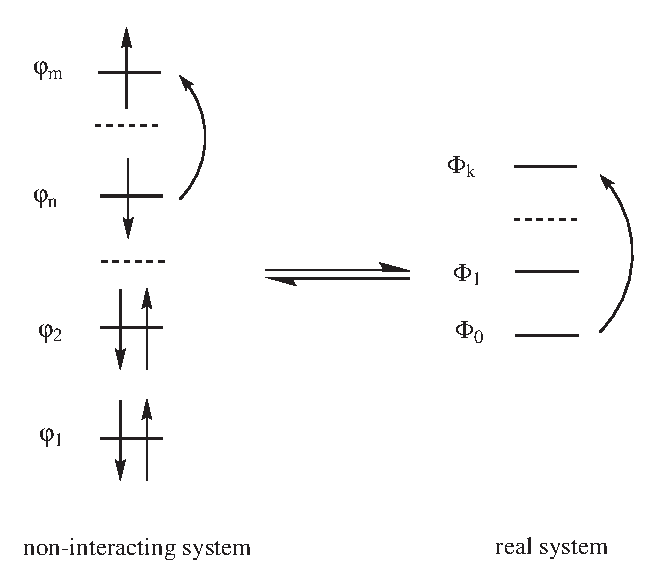
\includegraphics[scale=0.7]{TDexcitation.eps}
\caption{one to one correspondence  of electron excitation tween
non-interacting system and real system}\label{TDDFT:2}
\end{center}
\end{figure}



%%%%%%%%%%%%%%%%%%%%%%%%%%%%%%%%%%%%%%%%%%%%%%%%%%%%%%%%%%%%%%%%%%%%%%
\section{Linear response equation based on density matrix}
%
%
%
%
Now let's follow Casida's derivation for the linear response equation
on density matrix\footnote{see the reference of \cite{Casida1}}.
Suggest for some ground state of $\Psi_{0}$, some time dependent
perturbation is turning on:
\begin{equation}
 \label{TDDFT_Casida:1}
\delta \hat{v} (t) = \sum_{ij\sigma} \delta
v_{ij\sigma}(t)\hat{a}^{+}_{i\sigma}\hat{a}_{j\sigma} 
\end{equation} 
Here the $\hat{a}^{+}_{i\sigma}$ and $\hat{a}_{j\sigma}$ are two
annihilation operators used in second quantization theory. They
characterize that in orbital of $i$ some particle with spin of
$\sigma$ is destroyed and in the orbital $j$ this particle is
created. the $\delta v_{ij\sigma}(t)$ is some time dependent
perturbation that cause the $i$ and $j$ to have such changes. If it
goes over all the $i$ and $j$ pairs then we can use it to represent
the whole perturbation of $\delta \hat{v} (t)$ (compared with the
ordinary notion, in second quantization method we concentrate on the
generation and destruction of the particles, which is equivalent to
the changing of position variables).

What's more, the perturbed density matrix between orbital $i$ and $j$
can be expressed as:
\begin{equation}
 \label{TDDFT_Casida:2}
\delta P_{ij\sigma} (t) =
\bra{\delta
\Psi_{0}}\hat{a}^{+}_{i\sigma}\hat{a}_{j\sigma}\ket{
\Psi_{0}} + \bra{
\Psi_{0}}\hat{a}^{+}_{i\sigma}\hat{a}_{j\sigma}\ket{\delta
\Psi_{0}}
\end{equation} 

Now both of the $\delta P_{ij\sigma} (t)$ and $\delta v_{ij\sigma}
(t)$ can be associated with each other through some general
density kernel of $\chi_{ij\sigma, kl\tau}$:
\begin{equation}
  \label{TDDFT_Casida:3}
\delta P_{ij\sigma} (t) = \sum_{kl\tau}\int \chi_{ij\sigma, kl\tau}(t
- t^{'}) \delta v_{kl\tau} (t^{'}) dt^{'}
\end{equation} 
The (\ref{TDDFT_Casida:3}) it means that if we have some perturbation
switched on between $k$ and $l$ orbitals at time $t^{'}$ then it will
also cause the changes on the $i$ and $j$ pairs at the time $t$. Then
if we want to get the $\delta P_{ij\sigma} (t)$, we have to sum over
all the $k$ and $l$ pairs and goes over all the time space.

Here the expression above is actually identical with the analysis in
(\ref{TDDFT1}), where we have introduced the expression
from (\ref{TDDFTeq:45}) to (\ref{TDDFTeq:23}). Here the most
important distinguishment is that in the second quantization
representation the density kernel is concentrated on the particles
rather than the position variables compared with the
(\ref{TDDFTeq:29}) and (\ref{TDDFTeq:23}). However,
they are identical with each other.

Based on the (\ref{TDDFT_Casida:3}), by using the Fourier
transformation, the above expression can be transformed
into frequency space:
\begin{align}
   \label{TDDFT_Casida:8}
\delta P_{ij\sigma} (\omega) &= \sum_{kl\tau} \chi_{ij\sigma,
kl\tau}(\omega) \delta v_{kl\tau} (\omega ) 
\end{align}

From perturbation treatment, we can get the $\chi$
expression in the traditional wave function method, which is
identical to the (\ref{TDDFTeq:28}):
\begin{multline}\label{TDDFT_Casida:4}
\chi_{ij\sigma, kl\sigma^{'}}(\omega) =
\lim_{\eta \rightarrow 0^{+}}\sum_{m > 0}\left\{
\frac{\bra{0}\hat{a}^{+}_{i\sigma}\hat{a}_{j\sigma^{'}}\ket{m}
      \bra{m}\hat{a}^{+}_{k\sigma}\hat{a}_{l\sigma^{'}}\ket{0}}
      {\omega - (E_{m} - E_{0})+ i\eta}
      \right. - \\
\left. 
\frac{\bra{0}\hat{a}^{+}_{k\sigma}\hat{a}_{l\sigma^{'}}\ket{m}
      \bra{m}\hat{a}^{+}_{i\sigma}\hat{a}_{j\sigma^{'}}\ket{0}}
      {\omega + (E_{m} - E_{0})+ i\eta}
\right\}
\end{multline}

for the non-interacting system, in the gound sate we have some single
particle equation:
\begin{equation}
 \label{TDDFT_Casida:5}
\hat{h}\psi_{i\sigma} = \epsilon_{i\sigma}\psi_{i\sigma}
\end{equation} 
Here $\psi_{i\sigma}$ is the Kohn-Sham orbital, and it assumes that
we use the orthogonal basis sets. Based on this special case, the
density kernel in the (\ref{TDDFT_Casida:4}) can be expressed
as:
\begin{align}
  \label{TDDFT_Casida:7}
\chi_{ij\sigma, kl\sigma^{'}}(\omega) &=
\delta_{\sigma\sigma^{'}}\delta_{ik}\delta_{jl}\frac{
f_ { j\sigma} -
f_{i\sigma}}{\omega - (\epsilon_{i\sigma} - \epsilon_{j\sigma})}
\end{align} 
The $f_{i\sigma}$ indicates the occupation number on the orbitals (so
the orbials has been classified into virtual and occupied type).

the expression in the (\ref{TDDFT_Casida:7}) combined with
(\ref{TDDFT_Casida:8}) are our foundation for further discussion. 

%%%%%%%%%%%%%%%%%%%%%%%%%%%%%%%%%%%%%%%%%%%%%%%%%%%%%%%%%%%%%%%%%%%%%
\subsection{Linear response of the density matrix}
%
%
%
%
%
Suggest that for some ground state non-interacting system some time
dependent filed is switched on, then the perturbation in first order
for the Kohn-Sham Hamiltonian can be expressed as:
\begin{equation}
 \label{TDDFT_Casida:9}
\delta v_{eff}(r,t) =  v_{ext}(r,t) + \delta v_{KS}(r,t)
\end{equation} 
Here because of the adding of external potential of $v_{ext}(r,t)$,
the ground state density will change so accordingly, the ground state
Kohn-Sham potential of $v_{KS}$ will be altered. Hence, from the
(\ref{TDDFT_Casida:8}) we can express such relation as:
\begin{align}
\label{TDDFT_Casida:10}
 \delta P_{ij\sigma} (\omega) &= \sum_{kl\tau} \chi_{ij\sigma,
kl\tau}(\omega) \delta v^{eff}_{kl\tau} (\omega ) \nonumber \\
&=
\sum_{kl\tau} 
\delta_{\sigma\tau}\delta_{ik}\delta_{jl}\frac{f_{j\sigma} -
f_{i\sigma}}{\omega - (\epsilon_{i\sigma} - \epsilon_{j\sigma})}
\delta v^{eff}_{kl\tau} (\omega ) \nonumber \\
&= \frac{f_{j\sigma} - f_{i\sigma}}{\omega - (\epsilon_{i\sigma} -
\epsilon_{j\sigma})}
\delta v^{eff}_{ij\sigma} (\omega )
\end{align} 
Here, we can see that for the $f_{j\sigma} = f_{i\sigma}$, the first
order density matrix change is zero. It implies that only the pair of
virtual-occupied orbitals are making contribution to the first order
density. The virtual-virtual pair and occupied-occupied pair are all
goes to be zero. This character is important in the following
linear response equation establishment.

On the other hand, from the above analysis we can see that $\delta
v_{KS}(\omega)$ is also dependent on the changing of density (so as
the density matrix), hence we can express such relation as:
\begin{equation}
 \label{TDDFT_Casida:11}
\delta v^{KS}_{ij\sigma} (\omega) = \sum_{kl\tau}K_{ij\sigma,
kl\tau}(\omega) \delta P_{kl\tau} (\omega) 
\end{equation}  

Let's bring the (\ref{TDDFT_Casida:11}) into the
(\ref{TDDFT_Casida:10}) so that to eliminate the $\delta
v^{KS}_{ij\sigma} (\omega)$, then we can have:
\begin{equation}
  \frac{\omega - (\epsilon_{i\sigma} -
\epsilon_{j\sigma})}{f_{j\sigma} - f_{i\sigma}}
\delta P_{ij\sigma} (\omega) = v_{ext}(\omega) +
\sum_{kl\tau}K_{ij\sigma,
kl\tau}(\omega) \delta P_{kl\tau} (\omega)
\end{equation} 
Then let's merge the density matrix together, then we have:
\begin{equation}
\begin{split}
\label{TDDFT_Casida:12}
&\sum_{kl\sigma^{'}}^{f_{j\sigma} \neq f_{i\sigma}}  
\Bigg\{
\delta_{\sigma\sigma^{'}}\delta_{ik}\delta_{jl}
\frac{
\omega - (\epsilon_{k\sigma^{'}} - \epsilon_{l\sigma^{'}})}
{f_{l\sigma^{'}} - f_{k\sigma^{'}}}
-
K_{ij\sigma,
kl\sigma^{'}}(\omega)
\Bigg\}
\delta P_{kl\sigma^{'}} (\omega) \\
&= v_{ext}(\omega)
\end{split} 
\end{equation}
Now we have arrived at some equation, this fundamental equation
associates the frequency and the density matrix together, later we
will build the real linear response equation from this point.
However, so far let's first analyze the four index variable of
$K_{ij\sigma, kl\sigma^{'}}(\omega)$ first. 


%%%%%%%%%%%%%%%%%%%%%%%%%%%%%%%%%%%%%%%%%%%%%%%%%%%%%%%%%%%%%%%%%%%%%
\subsection{The coupling matrix}
\label{sec:coupling_matrix_in_TDDFT}
%
%
%
%
%
The $K_{ij\sigma, kl\sigma^{'}}(\omega)$ appeared in the function of
(\ref{TDDFT_Casida:12}) is actually called ``coupling matrix'', which
is defined in (\ref{TDDFT_Casida:11}):
\begin{equation}
\delta v^{KS}_{ij\sigma} (\omega) = \sum_{kl\tau}K_{ij\sigma,
kl\tau}(\omega) \delta P_{kl\tau} (\omega) 
\end{equation}
Hence we can calculate it as:
\begin{equation}
 K_{ij\sigma, kl\tau}(\omega) = \frac{\partial v^{KS}_{ij\sigma}
(\omega)}{\partial P_{kl\tau} (\omega)}
\end{equation} 
By the chain rule for the partial derivative, we can get:
\begin{align}
\label{TDDFT_Casida:13}
  K_{ij\sigma, kl\tau}(\omega) &=\int^{+\infty}_{-\infty}
e^{i\omega(t-t^{'})} \frac{\partial v^{KS}_{ij\sigma}
(t)}{\partial P_{kl\tau} (t^{'})} d(t-t^{'}) \nonumber \\
&= \int^{+\infty}_{-\infty}
e^{i\omega(t-t^{'})} \Bigg\{ 
\sum_{\mu}\int 
\frac{\delta v^{KS}_{ij\sigma}(t)}
{\delta \rho_{\mu} (r^{'}, t^{''})}
\frac{\partial\rho_{\mu} (r^{'},t^{''})}{\partial P_{kl\tau} (t^{'})}
d^{3}r^{'}dt^{''}
 \Bigg\} d(t-t^{'}) \nonumber \\
&=
(\varphi^{*}_{i\sigma}\varphi_{j\sigma}|\varphi^{*}_{k\tau}\varphi_{
l\tau}) + \int^{+\infty}_{-\infty}
e^{i\omega(t-t^{'})} \nonumber \\
&\Bigg\{
\int
\varphi^{*}_{i\sigma}(r)\varphi_{j\sigma}(r)  
\frac{\delta^{2} E_{XC}}
{\delta \rho_{\sigma} (r, t)\delta \rho_{\tau} (r^{'}, t^{'})}
\varphi^{*}_{k\tau}(r^{'})\varphi_{l\tau}(r^{'})
d^{3}r^{'}d^{3}r
\Bigg\} d(t-t^{'})
\end{align}

If we apply the adiabatic approximation(see \ref{TDDFT_EXC_eq:2}),
then we can have the second term indepdent of time:
\begin{multline}
\int^{+\infty}_{-\infty}
e^{i\omega(t-t^{'})} \Bigg\{
\int
\varphi^{*}_{i\sigma}(r)\varphi_{j\sigma}(r)\\
\shoveleft{  
\frac{\delta^{2} E_{XC}}
{\delta \rho_{\sigma} (r, t)\delta \rho_{\tau} (r^{'}, t^{'})}
\varphi^{*}_{k\tau}(r^{'})\varphi_{l\tau}(r^{'})
d^{3}r^{'}d^{3}r
\Bigg\} d(t-t^{'})}  \\
= \int
\varphi^{*}_{i\sigma}(r)\varphi_{j\sigma}(r)  
\frac{\delta^{2} E_{XC}}
{\delta \rho_{\sigma} (r)\delta \rho_{\tau} (r^{'})}
\varphi^{*}_{k\tau}(r^{'})\varphi_{l\tau}(r^{'})
d^{3}r^{'}d^{3}r
\end{multline} 
This is what we have got in the previous section. Hence finally, the
coupling matrix is expressed as:
\begin{align}
\label{TDDFT_Casida:14}
 K_{ij\sigma, kl\tau}(\omega) &=
(\varphi^{*}_{i\sigma}\varphi_{j\sigma}|\varphi^{*}_{k\tau}\varphi_{
l\tau}) + \nonumber \\
&\int
\varphi^{*}_{i\sigma}(r)\varphi_{j\sigma}(r)  
\frac{\delta^{2} E_{XC}}
{\delta \rho_{\sigma} (r)\delta \rho_{\tau} (r^{'})}
\varphi^{*}_{k\tau}(r^{'})\varphi_{l\tau}(r^{'})
d^{3}r^{'}d^{3}r
\end{align}

%%%%%%%%%%%%%%%%%%%%%%%%%%%%%%%%%%%%%%%%%%%%%%%%%%%%%%%%%%%%%%%%%%%%%
\subsection{Structure for linear response equation}
\label{TDDFT:1}
%
%
%
%
%
As what has been demonstrated in the (\ref{TDDFT_Casida:10}), only
the occ-vir pair blocks exists in the expression of density matrix.
Hence for more clear specification, let's follow the convention
that the subscript of $i,j, k$ etc. indicate the occupied orbitals,
$a, b, c$ etc. represent the virtual orbitals; and $p, q, r$ etc.
refer to the general orbitals.
Based on this point, the result in the (\ref{TDDFT_Casida:12}) can be
rewritten as:
\begin{equation}
\label{TDDFT_Casida:18} 
 \begin{split}
  &\sum_{j}\sum_{b}\sum_{\sigma^{'}}\left\lbrace 
\delta_{\sigma\sigma^{'}}\delta_{ij}\delta_{ab}\left[ 
\frac{\omega - (\epsilon_{i} - \epsilon_{a})}{f_{a} -
f_{i}} \right] 
- K_{ia\sigma,
jb\sigma^{'}}(\omega)
\right\rbrace 
\delta P_{jb\sigma^{'}} (\omega) \\
&- \sum_{b}\sum_{j}\sum_{\sigma^{'}}K_{ia\sigma,
bj\sigma^{'}}(\omega)\delta P_{bj\sigma^{'}} (\omega)
= v_{ext}(\omega)
 \end{split}
\end{equation} 
this function is for some pre-determined occ-vir pair of $ia\sigma$ in
the $K_{ia\sigma, jb\sigma^{'}}$. Compared with the
(\ref{TDDFT_Casida:12}), we have such index correspondence:
\begin{align}
 i \leftrightarrow i  &\quad  j \leftrightarrow a \quad
(\text{pre-determined pairs}) \nonumber \\
 k \leftrightarrow j  &\quad  l \leftrightarrow b \quad
(\text{the first term}) \nonumber \\
 k \leftrightarrow b  &\quad  l \leftrightarrow j \quad
(\text{the second term}) \nonumber \\
\end{align} 

However, for the pre-determined pair of $ai\sigma$, we can have some
conjugated equation (derived in the same way):
\begin{equation}
\label{TDDFT_Casida:19} 
  \begin{split}
  &\sum_{b}\sum_{j}\sum_{\sigma^{'}}\left\lbrace 
\delta_{\sigma\sigma^{'}}\delta_{ij}\delta_{ab}\left[ 
\frac{\omega - (\epsilon_{a} - \epsilon_{i})}{f_{i} -
f_{a}} \right] 
- K_{ai\sigma,
bj\sigma^{'}}(\omega)
\right\rbrace 
\delta P_{bj\sigma^{'}} (\omega) \\
&- \sum_{j}\sum_{b}\sum_{\sigma^{'}}K_{ai\sigma,
jb\sigma^{'}}(\omega)\delta P_{jb\sigma^{'}} (\omega)
= v_{ext}(\omega)
 \end{split}
\end{equation} 

Now let's try to combine them together to form the final equation.
Firstly, we notice that (this is obvious from the definition of
density matrix): 
\begin{equation}
\label{TDDFT_Casida:16}
 \delta P_{jb\sigma^{'}} (\omega) = \delta P^{*}_{bj\sigma^{'}}
(\omega)
\end{equation}
Moreover, let's deal with the left side of matrix element:
\begin{equation}
\label{TDDFT_Casida:17} 
\begin{split}
 A_{ia\sigma, jb\sigma^{'}} &=
\delta_{\sigma\sigma^{'}}\delta_{ij}\delta_{ab}\left[ 
\frac{(\epsilon_{i} - \epsilon_{a})}{f_{a} -
f_{i}} \right] 
+ K_{ia\sigma, jb\sigma^{'}}(\omega) \\
&=\delta_{\sigma\sigma^{'}}\delta_{ij}\delta_{ab}(\epsilon_{a} -
\epsilon_{i}) + K_{ia\sigma, jb\sigma^{'}}(\omega) 
\end{split}
\end{equation}  
Here we have to remember that $f_{a} = 0$ and $f_{i} = 1$.
Hence the first equation in (\ref{TDDFT_Casida:18}) is
converted to be:
\begin{equation}
 \label{TDDFT_Casida:20}
-\omega \delta P_{ia\sigma} (\omega) - v_{ext}(\omega) = 
\sum_{j}\sum_{b}\sum_{\sigma^{'}}A_{ai\sigma, jb\sigma^{'}}\delta
P_{jb\sigma^{'}}
(\omega) + K_{ai\sigma, bj\sigma^{'}}\delta P_{bj\sigma^{'}}(\omega)
\end{equation} 

The conjugatedequation can be rewriten as:
\begin{equation}
 \label{TDDFT_Casida:21}
\omega \delta P_{ai\sigma} (\omega) - v_{ext}(\omega) = 
\sum_{j}\sum_{b}\sum_{\sigma^{'}}A_{ia\sigma, jb\sigma^{'}}\delta
P_{jb\sigma^{'}}
(\omega) + K_{ia\sigma, bj\sigma^{'}}\delta P_{bj\sigma^{'}}(\omega)
\end{equation} 

Finally, let's introduce the ``zero frequency limit'' which is
usually used in deriving the final equation; that is to say,
$v_{ext}(\omega)$ can be set to $0$. Thus we can set the
$v_{ext}(\omega)$ into zero. Hence the final linear equation is:
\begin{equation}
 \label{TDDFT_Casida_final:1}
-\omega \delta P_{ia\sigma} (\omega)  = 
\sum_{j}\sum_{b}\sum_{\sigma^{'}}A_{ai\sigma, jb\sigma^{'}}\delta
P_{jb\sigma^{'}}
(\omega) + K_{ai\sigma, bj\sigma^{'}}\delta P_{bj\sigma^{'}}(\omega)
\end{equation} 

The conjugatedequation can be rewriten as:
\begin{equation}
 \label{TDDFT_Casida_final:2}
\omega \delta P_{ai\sigma} (\omega)  = 
\sum_{j}\sum_{b}\sum_{\sigma^{'}}A_{ia\sigma, jb\sigma^{'}}\delta
P_{jb\sigma^{'}}
(\omega) + K_{ia\sigma, bj\sigma^{'}}\delta P_{bj\sigma^{'}}(\omega)
\end{equation} 
They are same with the equations we got in the
(\ref{TTDFT_ENERGY_TFLRE}).


%%%%%%%%%%%%%%%%%%%%%%%%%%%%%%%%%%%%%%%%%%%%%%%%%%%%%%%%%%%%%%%%%%%%%%
\section{Gordon's way to derive the linear response equation}
%
%
%
%
In the previous content, we have presented two ways to derive to
linear response equation, both of them are given in the complete and
detailed way. However, the two above derivations share a same
character, that is they are all based upon the perturbation on KS
orbitals. Their difference, is that the Gross's derivation is based
on the electron density (so we use the functional and functional
derivatives to connect the perturbed density, Hamiltonian etc.), but
Cacida use the density matrix to rewrite the whole expression (hence
the expression is based on the annihilation operator, so we get
different expression for the density response kernel). However, the
physical idea is same among the two way of derivations. However, all
of them are based on the MO representation, that's what they share in
common.

Now in this section we will present the third way to derive the
linear response equation\cite{Gordon, Hirata1999291}. The derivation
here is totally based on the perturbation of Fock matrix, rather
than the MO space-this is the essential distinguishment between this
method and the above methods. However, as what has been demonstrated;
the physical idea is shared between all of them.

%%%%%%%%%%%%%%%%%%%%%%%%%%%%%%%%%%%%%%%%%%%%%%%%%%%%%%%%%%%%%%%%%%%%%%
\subsection{Starting from TDKS equation}\label{Gordon_TDKS}
%
%
%
%
Let's from the matrix form of TDKS (time dependent Kohn-Sham)
equation, which has been discussed in detail at the section
\ref{TDKS_equation}. We are starting from the equation
(\ref{TDDFTeq:21}):
\begin{equation}\label{Grodon_TDDFT_equation:1}
i \frac{\partial P_{pr}}{\partial t} =
\sum_{q}\left\{F_{pq}P_{qr} -
P_{pq}F_{qr}\right\}
\end{equation}
Here the $P_{pq}$ is the density matrix between the basis set
functions of $\psi_{p}(r)$ and $\psi_{q}(r)$:
\begin{equation}
 \label{Grodon_TDDFT_equation:2}
\rho(r) = \sum_{pq}P_{pq}\psi^{*}_{p}(r)\psi_{q}(r)
\end{equation} 
Here the basis set function is the KS orbital describing the ground
state of the system.

On the other hand, the $F_{pq}$ is the Fock matrix for the basis set
functions and the time-dependent Kohn-sham Hamiltonian (as defined
in the \ref{TDDFTeq:17}):
\begin{multline}
\label{Grodon_TDDFT_equation:3}
F_{pq} = 
\int d^{3}r\psi^{*}_{p}(r)\left\{ -\frac{1}{2}\nabla^{2} + v(r,t) +
\int d^{3}r^{'}\frac{\rho(r^{'}, t)}{|r-r^{'}|} \right. \\
\left. + \frac{\delta
E_{xc}[\rho(r,t)]}{\delta\rho(r,t)} \right\}\psi_{q}(r)
\end{multline}

Generally, as what we have always followed; to directly solve this
equation is very hard; hence we employ the perturbation treatment.
let's start from the ground state, since the Kohn-sham orbital are
all orthogonal with each other, we can have:
\begin{align}
 \label{Grodon_TDDFT_equation:4}
P^{0}_{pq} &= \delta_{pq} \nonumber \\
F^{0}_{pq} &= \epsilon_{q}\delta_{pq} 
\end{align}
Different with the (\ref{Grodon_TDDFT_equation:3}), the $F^{0}_{pq}$
here is only referred as the ground state Kohn-Sham Hamiltonian:
\begin{align}\label{Grodon_TDDFT_equation:12}
F^{0}_{pq} &= 
\int d^{3}r\psi^{*}_{p}(r)\left\{ -\frac{1}{2}\nabla^{2} +
\int d^{3}r^{'}\frac{\rho(r^{'}, t)}{|r-r^{'}|}  + \frac{\delta
E_{xc}}{\delta\rho(r)} \right\}\psi_{q}(r) \nonumber \\
&=\int d^{3}r\psi^{*}_{p}(r) F^{KS}\psi_{q}(r) \nonumber \\
&=\epsilon_{q}\int d^{3}r\psi^{*}_{p}(r)\psi_{q}(r) \nonumber \\
&=\epsilon_{q}\delta_{pq}
\end{align}
$\epsilon_{q}$ here is the orbital energy for the orbital $q$.

Now let's introduce the naming of the subscript, we use $p,q,r\cdots$
to designate the general orbitals, $i,j,k\cdots$ to denote the
occupied orbitals and $a,b,c\cdots$ to refer to the virtual orbitals.

For the ground state, since the density matrix of $P$ is invarient of
time change, then the equation (\ref{Grodon_TDDFT_equation:1})
becomes:
\begin{equation}\label{Grodon_TDDFT_equation:5}
\sum_{q}\left\{F^{0}_{pq}P^{0}_{qr} -
P^{0}_{pq}F^{0}_{qr}\right\} = 0
\end{equation}

Now suggest that some oscillatory perturbation is switched on (such
as the case in photochemistry), the external field can be expressed
as:
\begin{equation}\label{Grodon_TDDFT_equation:6}
v_{1}(r,t) = \frac{1}{2}\left[ f_{pq}e^{i\omega t} + f_{qp}e^{-i\omega
t}\right] 
\end{equation}
Here we have $f_{qp} = f^{*}_{pq}$ so that to ensure that the
perturbation operator is hermitian. Furthermore, we note that this
expression actually is consistent with the form in
(\ref{TDDFTeq:51}), we only extend the $E$ there as the $f_{pq}$ and
$f_{qp}$.

As the perturbation is switched on, then the density matrix of $P$ is
also changed:
\begin{equation}\label{Grodon_TDDFT_equation:7}
P_{pq} = P^{0}_{pq} + P^{1}_{pq}
\end{equation}
the $P^{1}_{pq}$ could be expressed as:
\begin{equation}\label{Grodon_TDDFT_equation:8}
P^{1}_{pq} = \frac{1}{2}\left[ d_{pq}e^{i\omega t} + d_{qp}e^{-i\omega
t}\right] 
\end{equation}

For the Fock matrix, the corresponding change can be expressed as:
\begin{equation}\label{Grodon_TDDFT_equation:9}
F_{pq} = F^{0}_{pq} + G_{pq} + F^{1}_{pq}
\end{equation}
$G_{pq}$ is referred as the Fock matrix for the $v_{1}(r,t)$:
\begin{equation}
\label{Grodon_TDDFT_equation:10}
G_{pq} = \int d^{3}r v_{1}(r,t)\psi^{*}_{p}(r)\psi_{q}(r)
\end{equation} 
and $F^{1}_{pq}$ could be expressed as:
\begin{equation}\label{Grodon_TDDFT_equation:11}
F^{1}_{pq} = \sum_{rs}\frac{\partial F_{pq}}{\partial
P_{rs}}P^{1}_{rs} 
\end{equation}

The expression in (\ref{Grodon_TDDFT_equation:9}) actually can be
easily understood. Suggest we have some function of $f(x)$, then the
differential of $f(x)$ is:
\begin{equation}
 df(x) = f'(x)dx
\end{equation}
Hence the $f(x) + df(x)$ just corresponds the little change for
$f(x)$ at the certian point of $x$, thus we can have the
similarities:
\begin{align}
 f(x) + df(x) &\leftrightarrow F_{pq} \nonumber \\
        df(x) &\leftrightarrow F^{1}_{pq} \nonumber \\
        f'(x) &\leftrightarrow \frac{\partial F_{pq}}
                                {\partial P_{rs}} \nonumber \\
        dx &\leftrightarrow  P^{1}_{rs}
\end{align}
Certainly we have to remember here that the Fock matrix is the
multivariate function for density matrix.

%%%%%%%%%%%%%%%%%%%%%%%%%%%%%%%%%%%%%%%%%%%%%%%%%%%%%%%%%%%%%%%%%%%%%%
\subsection{Further discussion for $F^{1}_{pq}$}
%
%
%
%
%
Now let's stop for a little while and go to see the details for the
$F^{1}_{pq}$, the problem is; whether this express can correspond to
the coupling matrix (Actually, judging from the appearance, it
should be)?

Let's suggest that the exchange correlation energy can be expressed
as:
\begin{equation}
 E_{XC} = \int L(r) d^{3}r
\end{equation}
Then the Fock matrix expressed in the
(\ref{Grodon_TDDFT_equation:12}) is actually:
\begin{equation}
\label{Grodon_TDDFT_equation:13}
 F^{0}_{pq} = \int d^{3}r\int d^{3}r^{'}\psi^{*}_{p}(r)
\frac{\rho(r^{'})}{|r-r^{'}|}
\psi_{q}(r) + \int d^{3}r
v_{xc}(r)\psi^{*}_{p}(r)\psi_{q}(r)
\end{equation} 
Hence we can get:
\begin{align}
 \label{Grodon_TDDFT_equation:14}
\frac{\partial F_{pq}}{\partial
P_{rs}}
&= \int d^{3}r\int d^{3}r^{'}\psi^{*}_{p}(r)\frac{\partial\left( 
\frac{\rho(r^{'})}{|r-r^{'}|}\right) }{\partial P_{st}}
\psi_{q}(r) + \int d^{3}r
\frac{\partial v_{xc}(r)}{\partial P_{st}}\psi^{*}_{p}(r)\psi_{q}(r)
\nonumber \\
&= \int d^{3}r\int d^{3}r^{'}
\psi^{*}_{s}(r^{'})\psi_{t}(r^{'})
\frac{1}{|r-r^{'}|}
\psi^{*}_{p}(r)\psi_{q}(r) \nonumber \\
&+
\int d^{3}r\int d^{3}r^{'}
\frac{\delta v_{xc}(r)}{\delta \rho(r^{'})}\frac{\partial
\rho(r^{'})}{\partial P_{st}}\psi^{*}_{p}(r)\psi_{q}(r)
\nonumber \\
&= (\psi_{p}\psi_{q}|\psi_{s}\psi_{t}) + \int d^{3}r\int d^{3}r^{'}
\psi^{*}_{p}(r)\psi_{q}(r)
\frac{\delta^{2} L (r)}{\delta \rho(r)\delta
\rho(r^{'})}\psi^{*}_{s}(r)\psi_{t}(r)
\end{align}
Now compared with the coupling matrix in the secion 
\ref{sec:coupling_matrix_in_TDDFT}, this is just the $K_{pq,st}$. The
only thing is that we have not taken spin into account.

%%%%%%%%%%%%%%%%%%%%%%%%%%%%%%%%%%%%%%%%%%%%%%%%%%%%%%%%%%%%%%%%%%%%%%
\subsection{Spin consideration}
%
%
%
Now let's take spin into consideration. Since for the ground state KS
equation, the $P^{0}_{pq}$ and $F^{0}_{pq}$ are all for pure spin
state:
\begin{align}
  \label{Grodon_TDDFT_equation:15}
P^{0}_{p\sigma,q\tau} &= \delta_{\sigma\tau}\delta_{pq} \nonumber \\
F^{0}_{p\sigma,q\tau} &= \epsilon_{q}\delta_{\sigma\tau}\delta_{pq}
\end{align}
Hence we can label them as $P^{0}_{pq\sigma}$ and $F^{0}_{pq\sigma}$.

For the $F^{1}_{pq}$, the response for the density matrix should take
into both of the spin states, so that it gives:
\begin{align}
   \label{Grodon_TDDFT_equation:16}
F^{1}_{pq\sigma} = \sum_{\tau}\sum_{rs}\frac{\partial
F^{0}_{pq\sigma}}{\partial
P_{rs\tau}}P^{1}_{rs\tau} 
\end{align}
And for the $P^{1}_{pq}$, as for well known fact that it only exists
for the occupied-virtual blocks and it's also the pure spin state:
\begin{equation}
  \label{Grodon_TDDFT_equation:17}
P^{1}_{pq\sigma} = 
\begin{cases}
0 & p=i, q= j \\
0 & p=a, q= b \\
\neq 0 & p=a, q = i \quad \text{or} \quad p = j, q = b              
\end{cases}
\end{equation} 

%%%%%%%%%%%%%%%%%%%%%%%%%%%%%%%%%%%%%%%%%%%%%%%%%%%%%%%%%%%%%%%%%%%%%%
\subsection{Linear response equation}
%
%
%
Finally, let's bring the (\ref{Grodon_TDDFT_equation:15}),
(\ref{Grodon_TDDFT_equation:16}) and 
(\ref{Grodon_TDDFT_equation:17}) as well as the corresponding
expression in section \ref{Gordon_TDKS} all into the equation
(\ref{Grodon_TDDFT_equation:1}), by collecting the terms multiplying
$e^{i\omega t}$ together, we can get some equation:
\begin{align}
 \label{Grodon_TDDFT_equation:18}
&F_{aa\sigma}P_{ai\sigma} - P_{ai\sigma}F_{ii\sigma} + \left\lbrace 
\sum_{st\tau}\left[\frac{\partial
F^{0}_{ai\sigma}}{\partial
P_{bj\tau}}P_{bj\tau} + \frac{\partial
F^{0}_{ai\sigma}}{\partial
P_{jb\tau}}P_{jb\tau} \right] 
+ g_{ai} \right\rbrace P^{0}_{ii\sigma} \nonumber \\
&=\omega P_{ai\sigma}
\end{align}

This function can be further simplified as:
\begin{align}
 \label{Grodon_TDDFT_equation:19}
&\left\lbrace 
\sum_{st\tau}\left[(\epsilon_{b} -
\epsilon_{j})
\delta_{ab}\delta_{ij}\delta_{\sigma\tau}P_{bj\tau} +
\frac{\partial
F^{0}_{ai\sigma}}{\partial
P_{bj\tau}}P_{bj\tau} + \frac{\partial
F^{0}_{ai\sigma}}{\partial
P_{jb\tau}}P_{jb\tau} \right] 
+ g_{ai} \right\rbrace \nonumber \\
&=\omega P_{ai\sigma}
\end{align}

By colleting the terms multiplying with $e^{-i\omega t}$, we can get
its pair equation:
\begin{align}
 \label{Grodon_TDDFT_equation:19}
&\left\lbrace 
\sum_{st\tau}\left[(\epsilon_{b} -
\epsilon_{j})
\delta_{ab}\delta_{ij}\delta_{\sigma\tau}P_{jb\tau} +
\frac{\partial
F^{0}_{ia\sigma}}{\partial
P_{bj\tau}}P_{bj\tau} + \frac{\partial
F^{0}_{ia\sigma}}{\partial
P_{jb\tau}}P_{jb\tau} \right] 
+ g_{ia} \right\rbrace \nonumber \\
&=-\omega P_{ia\sigma}
\end{align}

by neglecting the $g_{ia}$ and $g_{ai}$ at the zero frequency limit,
we can see the pair of equations are same with the final equations we
get in section (\ref{TTDFT_ENERGY_TFLRE}).

%%%%%%%%%%%%%%%%%%%%%%%%%%%%%%%%%%%%%%%%%%%%%%%%%%%%%%%%%%%%%%%%%%%%%%
\section{Singlet and triplet states}
%
%
%
Now let's made further discussion in terms of the spin. For the close
shell molecule its singlet and triplet excitation
can be expressed based on the density
matrix\cite{Bauernschmitt1996454}:
\begin{align}
 \label{TDDFT_singlet_triplet:0}
P_{ais} &= \frac{1}{\sqrt{2}}(P_{ai\alpha} + P_{ai\beta}) \nonumber \\
P_{ait} &= \frac{1}{\sqrt{2}}(P_{ai\alpha} - P_{ai\beta})
\end{align}
Here, ``s'' denotes the siglet state, and ``t'' is short for the
triplet state\footnote{For the origin of the singlet and triplet in
the TDDFT, please see the paper \cite{Gross8}. However, we should
note that there's no rigorous explanation for its origin}.
let's go to derive the concrete expression in terms of the spin state.

First of all, the general linear response equations are defined in
the (\ref{TDDFT_Casida_final:1}) and (\ref{TDDFT_Casida_final:2}),
which takes the form that:
\begin{equation}
 \label{TDDFT_singlet_triplet:1}
-\omega  P_{ia\alpha} (\omega)  = 
\sum_{j}\sum_{b}\sum_{\sigma}\left\lbrace A_{ai\alpha, jb\sigma}
P_{jb\sigma}
(\omega) + K_{ai\alpha, bj\sigma}
P_{bj\sigma}(\omega)\right\rbrace 
\end{equation}
and
\begin{equation}
 \label{TDDFT_singlet_triplet:2}
-\omega  P_{ia\beta} (\omega)  = 
\sum_{j}\sum_{b}\sum_{\sigma}\left\lbrace A_{ai\beta, jb\sigma}
P_{jb\sigma}
(\omega) + K_{ai\beta, bj\sigma}
P_{bj\sigma}(\omega)\right\rbrace 
\end{equation}

The corresponding pair equations are:
\begin{equation}
 \label{TDDFT_singlet_triplet:3}
\omega P_{ai\alpha} (\omega)  = 
\sum_{j}\sum_{b}\sum_{\sigma}A_{ia\alpha, jb\sigma}
P_{jb\sigma}(\omega) + K_{ia\alpha, bj\sigma}
P_{bj\sigma}(\omega)
\end{equation} 
and 
\begin{equation}
 \label{TDDFT_singlet_triplet:4}
\omega P_{ai\beta} (\omega)  = 
\sum_{j}\sum_{b}\sum_{\sigma}A_{ia\beta, jb\sigma}
P_{jb\sigma}(\omega) + K_{ia\beta, bj\sigma}
P_{bj\sigma}(\omega)
\end{equation} 

We starts from the two pair equations. Among them, the 
coupling matrix $K$ is defined as:
\begin{align}
\label{TDDFT_singlet_triplet:5}
 K_{ai\sigma, bj\tau}(\omega) &=
(\varphi^{*}_{a\sigma}\varphi_{i\sigma}|\varphi^{*}_{b\tau}\varphi_{
j\tau}) + \nonumber \\
&\int
\varphi^{*}_{a\sigma}(r)\varphi_{i\sigma}(r)  
\frac{\delta^{2} E_{XC}}
{\delta \rho_{\sigma} (r)\delta \rho_{\tau} (r^{'})}
\varphi^{*}_{b\tau}(r^{'})\varphi_{j\tau}(r^{'})
d^{3}r^{'}d^{3}r \nonumber \\
&=(ai|bj) + (ai|E^{XC}_{\sigma\tau}|bj)      
\end{align}
and the corresponding $A$ is:
\begin{equation}
\label{TDDFT_singlet_triplet:6}
 A_{ia\sigma, jb\sigma^{'}} 
=\delta_{\sigma\sigma^{'}}\delta_{ij}\delta_{ab}(\epsilon_{b} -
\epsilon_{j}) + K_{ia\sigma, jb\sigma^{'}}(\omega)
\end{equation}  

%%%%%%%%%%%%%%%%%%%%%%%%%%%%%%%%%%%%%%%%%%%%%%%%%%%%%%%%%%%%%%%%%%%%%%
\subsection{Properties for the coupling matrix}
%
%
%
%
Before we proceed on it's better for us to discuss a little bit more
about the prperties for the coupling matrix in terms of the spin
state.

As we have known, the coulomb matrix is invariant of the spin state.
For the exchange correlation part, since the second functional
derivatives is exchangeable:
\begin{equation}
\begin{split}
&\int
\varphi^{*}_{a\sigma}(r)\varphi_{i\sigma}(r)  
\frac{\delta^{2} E_{XC}}
{\delta \rho_{\sigma} (r)\delta \rho_{\tau} (r^{'})}
\varphi^{*}_{b\tau}(r^{'})\varphi_{j\tau}(r^{'})
d^{3}r^{'}d^{3}r \\
&= \int
\varphi^{*}_{a\sigma}(r)\varphi_{i\sigma}(r)  
\frac{\delta^{2} E_{XC}}
{\delta \rho_{\tau} (r^{'})\delta \rho_{\sigma} (r)}
\varphi^{*}_{b\tau}(r^{'})\varphi_{j\tau}(r^{'})
d^{3}r^{'}d^{3}r                 
\end{split}
\end{equation}  
Hence it's easily turned out that:
\begin{equation}
 (ai|E^{XC}_{\sigma\tau}|bj)   = 
(ai|E^{XC}_{\tau\sigma}|bj) = 
(ia|E^{XC}_{\sigma\tau}|bj) =
(ai|E^{XC}_{\sigma\tau}|jb) = 
(bj|E^{XC}_{\sigma\tau}|ai)      
\end{equation}
This property brings great feasibility for transforming the coupling
matrix. Hence finally, for the coupling matrix, we have:
\begin{equation}
\label{TDDFT_singlet_triplet:7}
K_{ai\sigma, bj\tau} = K_{bj\tau, ai\sigma}
= K_{ia\sigma, bj\tau} = K_{ai\sigma, jb\tau}
\end{equation}
 
For the matrix of $A$, compared with $K$ it's only have a redundant
term of $\delta_{\sigma\sigma^{'}}\delta_{ij}\delta_{ab}(\epsilon_{b}
-\epsilon_{j})$. However, we can see that this term is diagonal for
the block of $ai, bj$. Hence for the $A$ matrix we also have the
above equality\footnote{Here we have not considered the hybird
functional situation which requires the additional exchange term.
However, we can only merely add it in and it does not affect the
discussion here}:
\begin{equation}
\label{TDDFT_singlet_triplet:8}
A_{ai\sigma, bj\tau} = A_{bj\tau, ai\sigma}
= A_{ia\sigma, bj\tau} = A_{ai\sigma, jb\tau}
\end{equation}

%%%%%%%%%%%%%%%%%%%%%%%%%%%%%%%%%%%%%%%%%%%%%%%%%%%%%%%%%%%%%%%%%%%%%%
\subsection{Final expression}
%
%
%
%
Now according to the definition in (\ref{TDDFT_singlet_triplet:0}),
we can add (\ref{TDDFT_singlet_triplet:1}) and
(\ref{TDDFT_singlet_triplet:2}) together and multiply factor
$\frac{1}{\sqrt{2}}$ to each side, then we can get:
\begin{equation}
 \begin{split}
&-\omega  P_{ias} (\omega) \\
&=
\frac{1}{\sqrt{2}}\sum_{j}\sum_{b}\Big\{ \left[ 
\left( A_{ai\alpha, jb\alpha} + A_{ai\beta,
jb\alpha}\right)P_{jb\alpha} + 
\left( K_{ai\alpha, bj\alpha} +
K_{ai\beta, bj\alpha}\right)P_{bj\alpha} \right] + \\
&\left[ \left( A_{ai\alpha, jb\beta} + A_{ai\beta,
jb\beta}\right)P_{jb\beta}  +
\left( K_{ai\alpha, bj\beta} +
K_{ai\beta, bj\beta}\right)P_{bj\beta} \right] \Big\} 
 \end{split}
\label{TDDFT_singlet_triplet:9}
\end{equation} 

Now let's use the relation in (\ref{TDDFT_singlet_triplet:7}) and
(\ref{TDDFT_singlet_triplet:8}), this equality can be further
transformed as:
\begin{equation}
 \begin{split}
&-\omega  P_{ias} (\omega) \\
&=
\frac{1}{\sqrt{2}}\sum_{j}\sum_{b}\Big\{ \left[ 
\left( A_{ai\alpha, jb\alpha} + A_{ai\beta,
jb\alpha}\right)P_{jb\alpha} + 
\left( K_{ai\alpha, bj\alpha} +
K_{ai\beta, bj\alpha}\right)P_{bj\alpha} \right] + \\
&\left[ \left( A_{ai\alpha, jb\beta} + A_{ai\beta,
jb\beta}\right)P_{jb\beta}  +
\left( K_{ai\alpha, bj\beta} +
K_{ai\beta, bj\beta}\right)P_{bj\beta} \right] \Big\} 
 \end{split}
\label{TDDFT_singlet_triplet:10}
\end{equation} 


Firstly, we can use the spin symbol to specify the matrix function,
hence the function in (\ref{TDDFT_Casida_final:5}) is split into pair:
\begin{equation}\label{TDDFT_Casida_final:6}
\omega^{2} Z_{ai\alpha} 
= \sum_{j}\sum_{b}\sum_{\sigma}M_{ia\alpha, jb\sigma} Z_{bj\sigma}
\end{equation}
\begin{equation}\label{TDDFT_Casida_final:7}
\omega^{2} Z_{ai\beta} 
= \sum_{j}\sum_{b}\sum_{\sigma}M_{ia\beta, jb\sigma} Z_{bj\sigma}
\end{equation}
Here $\sigma$ goes over all the spin states, including the $\alpha$ and
$\beta$. 

Now let's multiply each of the equation with $(\sqrt{2})^{-1}$ and add
them together:
\begin{align}
 \omega^{2} \frac{1}{\sqrt{2}}(Z_{ai\alpha} + Z_{ai\beta})
&= \sum_{j}\sum_{b}\frac{1}{\sqrt{2}}(Z_{ai\alpha} +
Z_{ai\beta}) (M_{ia\alpha, jb\alpha} + M_{ia\alpha, jb\beta}\nonumber \\
& +M_{ia\beta, jb\alpha} +M_{ia\beta, jb\beta} ) \Rightarrow \nonumber
\\
\omega^{2} Z_{ais} &= \sum_{j}\sum_{b} Z_{bjs} (M_{ia\alpha, jb\alpha} +
M_{ia\alpha, jb\beta} +M_{ia\beta, jb\alpha} +M_{ia\beta, jb\beta} )
\end{align} 
In the siglet, since the $\rho_{\alpha} = \rho_{\beta}$, then we can
see that for the coupling matrix $K_{ia\sigma,
jb\sigma^{'}}(\omega)$, it has:
\begin{equation*}
 K_{ia\alpha, jb\beta}(\omega) = K_{ia\beta, jb\alpha}(\omega) \quad 
 K_{ia\alpha, jb\alpha}(\omega) = K_{ia\beta, jb\beta}(\omega)
\end{equation*}
for the term of
$\delta_{ij}\delta_{ab}\delta_{\sigma\sigma^{'}}(\epsilon_{a} -
\epsilon_{i})^{2}$, it's easily seen that this term cancelled in the
$\alpha$ and $\beta$ mixing case, and euqal to each other between the
$\alpha, \alpha$ and $\beta, \beta$ case. Hence we have the M matrix
element finally as:
\begin{multline}
 M_{ia\alpha, jb\alpha} +
M_{ia\alpha, jb\beta} +M_{ia\beta, jb\alpha} +M_{ia\beta, jb\beta} \\
= 
2\delta_{ij}\delta_{ab}(\epsilon_{a} - \epsilon_{i})^{2} + 
2(\epsilon_{a} - \epsilon_{i})^{\frac{1}{2}} 
(K_{ia\alpha, jb\alpha}(\omega) +
K_{ia\alpha, jb\beta}(\omega))(\epsilon_{b} -
\epsilon_{j})^{\frac{1}{2}}
\end{multline} 
The final matrix equation for the singlet is:
\begin{equation}
  \omega^{2}Z^{s} = M^{s}Z^{s}
\end{equation} 
With the element in $M^{s}$ is:
\begin{multline}
 M^{s}_{ia,jb} = 2\delta_{ij}\delta_{ab}(\epsilon_{a} -
\epsilon_{i})^{2} \\
+ (\epsilon_{a} - \epsilon_{i})^{\frac{1}{2}} 
(4(ia|jb) +2(ia|E^{\alpha\alpha}_{XC}|jb) + 
2(ia|E^{\alpha\beta}_{XC}|jb))(\epsilon_{b} -
\epsilon_{j})^{\frac{1}{2}}
\end{multline}

Simiarly, we can repeat the above procedure so that to produce the
triplet state (all the analysis are kept to be same, only pay attention
to the symbol change so some terms cancelled in the final expression):
\begin{equation}
  \omega^{2}Z^{t} = M^{t}Z^{t}
\end{equation} 
With the element in $M^{t}$ is:
\begin{equation}
 M^{t}_{ia,jb} = 2(\epsilon_{a} - \epsilon_{i})^{\frac{1}{2}} 
((ia|E^{\alpha\alpha}_{XC}|jb) - 
(ia|E^{\beta\beta}_{XC}|jb))(\epsilon_{b} -
\epsilon_{j})^{\frac{1}{2}}
\end{equation}




%%%%%%%%%%%%%%%%%%%%%%%%%%%%%%%%%%%%%%%%%%%%%%%%%%%%%%%%%%%%%%%%%%%%%%
\begin{comment}
%%%%%%%%%%%%%%%%%%%%%%%%%%%%%%%%%%%%%%%%%%%%%%%%%%%%%%%%%%%%%%%%%%%%%%



As what we have understand, the Fock matrix can be associated with
the functional potential:
\begin{align}
\label{TDDFT_TRANSFORMATION_EXC_KERNEL:1}
F^{\sigma}_{\mu\nu} &= \frac{\partial E^{\sigma}_{XC}}{\partial
P^{\sigma}_{\mu\nu}}
\nonumber \\
&=
\int \frac{\delta L(r)}{\delta
  \rho^{\sigma}(r)}\frac{\partial \rho^{\sigma}(r)}{\partial
P^{\sigma}_{\mu\nu}} d^{3}r
\nonumber \\
&= \int V^{\sigma}_{XC}(r) \phi^{*}_{\mu}(r)\phi_{\nu}(r) d^{3}r
\end{align}
Which is described in the (\ref{eq:XC_functional.9}). By the way, we
should remember that here the $P$ is referred to the ``density
matrix'' for the AO space not the pertubed density; for clarity, we
express the density matrix for the pertubed density as $Z$, that is
to say; $Z_{ai\sigma} = \delta P_{ai\sigma}$ in the above equations.

By the same procedure, we can evaluate the second derivatives:
\begin{align}
\label{TDDFT_TRANSFORMATION_EXC_KERNEL:2}
 \frac{\partial F^{\sigma}_{\mu\nu} }{\partial
P^{\sigma^{'}}_{\lambda\eta}} &= \int \frac{\delta 
F^{\sigma}_{\mu\nu}}
{\delta\rho_{\sigma^{'}}(r^{'})}\frac{\partial\rho_{\sigma^{'}}(r^{'})
}{
\partial
P^{\sigma^{'}}_{\lambda\eta}} d^{3}r^{'}
\nonumber \\ 
&= \int d^{3}r^{'} \frac{\delta 
F^{\sigma}_{\mu\nu}}
{\delta\rho_{\sigma^{'}}(r^{'})}\phi_{\lambda}
(r^{'})\phi_{\eta}(r^{'})
\nonumber \\ 
&= \int d^{3}r\int d^{3}r^{'}\phi^{*}_{\mu}(r)\phi_{\nu}(r)
\frac{\delta{V}^{\sigma}_{XC}(r)}{\delta\rho_{\sigma^{'}}(r^{'})}
\phi_{
\lambda} (r^{'})\phi_{\eta}(r^{'}) \nonumber \\
&= \int d^{3}r\int d^{3}r^{'}\phi^{*}_{\mu}(r)\phi_{\nu}(r)
\frac{\delta^{2}L(r)}{\delta\rho_{\sigma}(r)\delta\rho_{
\sigma^{'}}(r^{'})}
\phi_{
\lambda} (r^{'})\phi_{\eta}(r^{'})
\end{align}
The derivation here turns out that the exchange correlation kernel,
actually can be viewed as the susceptibility between the the pertubed
Fock Matrix $F_{\mu\nu}$ and pertubed $P_{\lambda\eta}$. Hence we
have: 
\begin{equation}
\begin{split}
&\sum_{ia\sigma}\sum_{kl\tau}Z_{ia\sigma}Z_{kl\tau}
\int\varphi^{*}_{i\sigma } (r)\varphi_{ j\sigma} (r) 
\frac{\delta^{2} E_{XC}}
{\delta \rho_{\sigma} (r)\delta \rho_{\tau} (r^{'})}
\varphi^{*}_{k\tau}(r^{'})\varphi_{l\tau}(r^{'})
d^{3}r^{'}d^{3}r \\
&= \sum_{\mu\nu}\sum_{\lambda\eta}\sum_{\sigma\tau}
P^{\sigma}_{\mu\nu} 
\frac{\partial F^{\sigma}_{\mu\nu}}{\partial
P^{\sigma^{'}}_{\lambda\eta}}P^{\sigma^{'}
}_{\lambda\eta} 
\end{split}
\end{equation}


Now let's go to see more details related to the final equation. The
equation shown in the (\ref{TDDFT_Casida_final:6}), actually can be
expanded as:
\begin{equation}
 \begin{split}
\omega^{2} Z_{ai\sigma} &=
\sum_{j}\sum_{b}\sum_{\sigma^{'}}M_{ia\sigma,
jb\sigma^{'}} Z_{bj\sigma^{'}}  \\
&= \sum_{jb\sigma^{'}}
\delta_{ij}\delta_{ab}\delta_{\sigma\sigma^{'}}(\epsilon_{a} -
\epsilon_{i})^{2}Z_{bj\sigma^{'}} + 2(\epsilon_{a} -
\epsilon_{i})^{\frac{1}{2}}K_{ia\sigma,
jb\sigma^{'}}(\omega)(\epsilon_{b} -
\epsilon_{j})^{\frac{1}{2}}Z_{bj\sigma^{'}} \\
&= (\epsilon_{a} -
\epsilon_{i})^{2}Z_{ai\sigma} + 2\sum_{jb\sigma^{'}}(\epsilon_{a} -
\epsilon_{i})^{\frac{1}{2}}\Big\{  (ia|jb) \\
&+(ia|E_{XC}^{\sigma\sigma^{'}}|jb) \Big\}(\epsilon_{b} -
\epsilon_{j})^{\frac{1}{2}}Z_{bj\sigma^{'}}
 \end{split}
\label{TDDFT_Casida_final:6}
\end{equation} 
Here the abbreviation is:
\begin{align}
 (ia|E^{\sigma\sigma^{'}}_{XC}|jb) &= \int d^{3}r \int d^{3}r^{'}
\varphi_{i}^{*}(r)\varphi_{a}(r)\frac{\partial^{2}
E_{XC}}{\partial \rho_{\sigma}(r)\partial \rho_{\sigma^{'}}(r^{'})}
\varphi_{j}^{*}(r^{'})\varphi_{b}(r^{'}) \nonumber \\
 (ia|jb) &= \int d^{3}r \int d^{3}r^{'} 
\varphi_{i}^{*}(r)\varphi_{a}(r) \frac{1}{r-r^{'}}
\varphi_{j}^{*}(r^{'})\varphi_{b}(r^{'}) 
\end{align}
$\varphi$ is the ground state Kohn-Sham orbitals.

Usually in practical coding, the calculation is usually transformed
back into the AO space (using the basis sets) while evaluating the
integrals, then back to the MO space (using molecular orbitals) while
forming the final matrix to calculate the linear response. Hence, how
can we transform it between the AO and MO? Let's concentrate on the
colomb integrals and the exchange-correlation integrals.

First, for the Colomb integral, it can be abbreviated as:
\begin{equation}
 J_{ia\sigma, jb\sigma^{'}} =
\sum_{jb\sigma^{'}}(ia|jb)Z_{bj\sigma^{'}}
\end{equation}  
Since the multiplier of energy differences are trivial to be added in
the final steps. For this integral, we can expand it into the AO as:
\begin{equation}
 \begin{split}
  J_{ia\sigma, jb\sigma^{'}} &=
\sum_{jb\sigma^{'}}\sum_{\mu\nu\lambda\eta}c^{*}_{i\mu}c_{a\nu}
c^{*}_{j\lambda}c_{b\eta}(\phi_{\mu}(r)\phi_{\nu}(r)|\phi_{\lambda}
(r^{'})\phi_{\eta}(r^{'}) )Z_{ bj\sigma^ {'}} \\
&=
\sum_{\mu\nu}c^{*}_{i\mu}c_{a\nu}\left\lbrace
\sum_{jb\sigma^{'}}\sum_{\lambda\eta}
c^{*}_{j\lambda}c_{b\eta}(\phi_{\mu}(r)\phi_{\nu}(r)|\phi_{\lambda}
(r^{'})\phi_{\eta}(r^{'}) )Z_{ bj\sigma^ {'}}\right\rbrace 
 \end{split}
\label{TDDFT_Casida_final:7}
\end{equation}  
Here we can see that the calculation within the curly bracket can be
calculated within the AO space. We notice that
$Z^{'}_{\lambda\eta} =
\sum_{jb\sigma^{'}}Z_{bj\sigma^{'}}c^{*}_{j\lambda}c_{b\eta}$ actually
forms some kind of new vector in the AO space. That's really what we
do
in AO calculation: first to make such transformation, then combined
with
the integral of
$(\phi_{\mu}(r)\phi_{\nu}(r)|\phi_{\lambda}(r^{'})\phi_{\eta}(r^{'}
))$
to give the result in AO space, then this result should be stored in
the $Z^{'}_{\mu\nu}$. Then we will finish the calculation in the AO
space. We note that here after the transformation of
$Z^{'}_{\lambda\eta}$, we can transform it back to the MO space by
$Z^{'}_{ai} = \sum_{\mu\nu}c^{*}_{i\mu}c_{a\nu} Z^{'}_{\mu\nu}$. Then
we
are back to the MO space and get the final result. Here the $Z^{'}$
vector is actually in dimension of $nbasis^{2}$.

Next let's talk about the the exchange-correlation part. Firstly,
let's
concentrate on the integral below:
\begin{equation}
 \begin{split}
&\sum_{jb\sigma^{'}} (ia|E_{XC}^{\sigma\sigma^{'}}|jb)
Z_{bj\sigma^{'}}
\\
&=\sum_{jb\sigma^{'}}\sum_{\mu\nu\lambda\eta}c^{*}_{i\mu}c_{a\nu}
c^{*}_{j\lambda}c_{b\eta}(\phi_{\mu}(r)\phi_{\nu}(r)|E_{XC}^{
\sigma\sigma^{'}}|\phi_{\lambda}
(r^{'})\phi_{\eta}(r^{'}) )Z_{ bj\sigma^ {'}} \\
&=\sum_{\mu\nu}c^{*}_{i\mu}c_{a\nu}\left\lbrace
\sum_{jb\sigma^{'}}\sum_{\lambda\eta}
c^{*}_{j\lambda}c_{b\eta}(\phi_{\mu}(r)\phi_{\nu}(r)|E_{XC}^{
\sigma\sigma^{'}}|\phi_{\lambda}
(r^{'})\phi_{\eta}(r^{'}) )Z_{ bj\sigma^ {'}}\right\rbrace 
 \end{split}
\label{TDDFT_Casida_final:8}
\end{equation} 
Here, we point out that the $(\phi_{\mu}(r)\phi_{\nu}(r)|E_{XC}^{
\sigma\sigma^{'}}|\phi_{\lambda} (r^{'})\phi_{\eta}(r^{'}) )$ is
actually the second partial derivatives for exchange correlation
energy with respect to the density matrix. In

Now let's combine the (\ref{TDDFT_Casida_final:8}),
(\ref{TDDFT_Casida_final:9}) and (\ref{TDDFT_Casida_final:10})
together, we can get the expression below:
\begin{equation}
 \begin{split}
  \sum_{jb\sigma^{'}} (ia|E_{XC}^{\sigma\sigma^{'}}|jb)
Z_{bj\sigma^{'}} = \sum_{\mu\nu}c^{*}_{i\mu}c_{a\nu}\left\lbrace
\sum_{jb\sigma^{'}}\sum_{\lambda\eta}
c^{*}_{j\lambda}c_{b\eta}Z_{ bj\sigma^
{'}} \frac{\partial^{2}
E_{XC}}{\partial P^{\sigma}_{\mu\nu}\partial
P^{\sigma^{'}}_{\lambda\eta}}\right\rbrace 
 \end{split}
\label{TDDFT_Casida_final:11}
\end{equation} 
Now, the same procedure can be done to the exchange correlation energy
again. Then we finish the transformation between the AO and MO.


%%%%%%%%%%%%%%%%%%%%%%%%%%%%%%%%%%%%%%%%%%%%%%%%%%%%%%%%%%%%%%%%%%%%%%
\section{Further derivation for the linear response equation}
%
%
%
%
Now let's approach to the final equation in some other
way\footnote{There seems to be something wrong with the matrix
representation, commonly used in many reference. just in the form
below:
\begin{equation}
 \omega 
\begin{bmatrix}
-1  &  0\\
 0  &  1
\end{bmatrix}
\begin{bmatrix}
  \delta P     \\
  \delta P^{*} \\
\end{bmatrix}
- v_{ext}(\omega)
= \begin{bmatrix}
  A & B \\
  B & A \\
\end{bmatrix}
\begin{bmatrix}
  \delta P     \\
  \delta P^{*} \\
\end{bmatrix} 
\end{equation} 
Here I want to mention that actually on the left side is the pure spin
state of $\delta P$, but on the right side we have added across over
all the spin states ($\sum\sigma^{'}$). So it cause some problems in
the further derivation. Hence I want to try another way to derive the
final equation. the original derivation is put into the final section
of this chapter}. 

First, we can simply add the equation in (\ref{TDDFT_Casida_final:1})
and (\ref{TDDFT_Casida_final:2}) together, which gives:
\begin{multline}
 \label{TDDFT_Casida_final:3}
\omega \left( \delta P_{ai\sigma} (\omega)-\delta P_{ia\sigma}
(\omega)\right) \\
= \sum_{j}\sum_{b}\sum_{\sigma^{'}}
\left[ ( A_{ia\sigma, jb\sigma^{'}} + B_{ia\sigma, jb\sigma^{'}})
(\delta P_{jb\sigma^{'}}(\omega) +
\delta P_{bj\sigma^{'}}(\omega))
\right] 
\end{multline}

On the other hand, we can make the (\ref{TDDFT_Casida_final:2}) and
(\ref{TDDFT_Casida_final:1}) substract each other, then it gives:
\begin{multline}
 \label{TDDFT_Casida_final:4}
\omega \left( \delta P_{ai\sigma} (\omega)+\delta P_{ia\sigma}
(\omega)\right) \\
= \sum_{j}\sum_{b}\sum_{\sigma^{'}}
\left[ ( A_{ia\sigma, jb\sigma^{'}} - B_{ia\sigma, jb\sigma^{'}})
(\delta P_{bj\sigma^{'}}(\omega) -
\delta P_{jb\sigma^{'}}(\omega))
\right] 
\end{multline}

Now let's observe the function of (\ref{TDDFT_Casida_final:4}). From
the (\ref{TDDFT_Casida:17}), we can see that 
\begin{equation*}
  A_{ia\sigma, jb\sigma^{'}} - B_{ia\sigma, jb\sigma^{'}} =
\delta_{\sigma\sigma^{'}}\delta_{ij}\delta_{ab}(\epsilon_{a} -
\epsilon_{i})
\end{equation*}
Let's bring it into the original function, it turns out:
\begin{align}
& \omega \left( \delta P_{ai\sigma} (\omega)+\delta P_{ia\sigma}
(\omega)\right) \nonumber \\
&= \sum_{j}\sum_{b}\sum_{\sigma^{'}}
\left[\delta_{\sigma\sigma^{'}}\delta_{ij}\delta_{ab}(\epsilon_{a} -
\epsilon_{i})
(\delta P_{bj\sigma^{'}}(\omega) -
\delta P_{jb\sigma^{'}}(\omega))
\right] \nonumber \\
&=  (\epsilon_{a} - \epsilon_{i}) (\delta P_{ai\sigma}(\omega) -
\delta P_{ia\sigma}(\omega))
\end{align} 
Now interestingly we can observe some very simple relationship between
the $(\delta P_{ai\sigma}(\omega) - \delta P_{ia\sigma}(\omega))$ and
the $(\delta P_{ai\sigma}(\omega) + \delta P_{ia\sigma}(\omega))$.
Here
we have such simple relation is because that the symmetrical property
of the coupling matrix. Then let's bring it back to the
(\ref{TDDFT_Casida_final:3}):
\begin{multline}
\frac{\omega^{2}}{\epsilon_{a} - \epsilon_{i}} \left( \delta
P_{ai\sigma} (\omega) + \delta P_{ia\sigma}
(\omega)\right) \\
= \sum_{j}\sum_{b}\sum_{\sigma^{'}}
\left[ ( A_{ia\sigma, jb\sigma^{'}} + B_{ia\sigma, jb\sigma^{'}})
(\delta P_{jb\sigma^{'}}(\omega) +
\delta P_{bj\sigma^{'}}(\omega))
\right] 
\end{multline} 
This is the final linear response equation. Here we can notice two
points: the first one is that the variables has been reduced into the
form of $\delta P_{ai\sigma} (\omega) + \delta P_{ia\sigma} (\omega)$.
Since $\delta P_{ai\sigma} (\omega) = \delta P^{*}_{ia\sigma}
(\omega)$, hence the index for the density matrix has been some real
number now! We have droped the complex number situation. Secondly, now
we only have one simple equation rather than a pair of equations
coupling with each other. 

Following the traditional transformation to the final function, let's
make some additional treatment. We can name some arbitrary variable of
$Z_{ai\sigma}$ as:
\begin{equation}
 Z_{ai\sigma} = \frac{1}{(\epsilon_{a} - \epsilon_{i})^{\frac{1}{2}}}
\left( \delta
P_{ai\sigma} (\omega) + \delta P_{ia\sigma}
(\omega)\right)
\end{equation} 
Hence the $\delta P_{jb\sigma^{'}}(\omega) +
\delta P_{bj\sigma^{'}}(\omega)$ on the right side of the equation can
be changed into:
\begin{equation}
 Z_{bj\sigma} = \frac{1}{(\epsilon_{b} - \epsilon_{j})^{\frac{1}{2}}}
\left( \delta P_{bj\sigma} (\omega) + \delta P_{jb\sigma}
(\omega)\right)
\end{equation}
Hence the final equation can be changed into:
\begin{equation}\label{TDDFT_Casida_final:5}
\omega^{2} Z_{ai\sigma} 
= \sum_{j}\sum_{b}\sum_{\sigma^{'}}\left[ (\epsilon_{a} -
\epsilon_{i})^{\frac{1}{2}}
 ( A_{ia\sigma, jb\sigma^{'}} + B_{ia\sigma, jb\sigma^{'}})
(\epsilon_{b} -
\epsilon_{j})^{\frac{1}{2}} \right] Z_{bj\sigma^{'}}
\end{equation}
This function just coincides with the result given in the Cacida's
paper\cite{Casida1}, although our derivation way is a bit of different
with his.

Finally let's expand the $A_{ia\sigma, jb\sigma^{'}} + B_{ia\sigma,
jb\sigma^{'}}$. It turns out that:
\begin{equation*}
A_{ia\sigma, jb\sigma^{'}} + B_{ia\sigma, jb\sigma^{'}} = 
\delta_{ij}\delta_{ab}\delta_{\sigma\sigma^{'}}(\epsilon_{a} -
\epsilon_{i}) + 2K_{ia\sigma,
jb\sigma^{'}}(\omega)
\end{equation*}
Hence the element inside the square bracket should be:
\begin{equation*}
 M_{ia\sigma, jb\sigma^{'}} =
\delta_{ij}\delta_{ab}\delta_{\sigma\sigma^{'}}(\epsilon_{a} -
\epsilon_{i})^{2} + 2(\epsilon_{a} -
\epsilon_{i})^{\frac{1}{2}}K_{ia\sigma,
jb\sigma^{'}}(\omega)(\epsilon_{b} -
\epsilon_{j})^{\frac{1}{2}}
\end{equation*} 
Hence we can introduce some new matrix of M, and obviously it's
symmetrical. Based on this new matrix, we can write the result
function
in the (\ref{TDDFT_Casida_final:5}):
\begin{equation}
\label{TDDFT_Casida_final:6}
 \omega^{2}Z = MZ
\end{equation} 
Here we should pay attention that the right side of the equation is
going over all the spin states.


%%%%%%%%%%%%%%%%%%%%%%%%%%%%%%%%%%%%%%%%%%%%%%%%%%%%%%%%%%%%%%%%%%%%%%
\section{New ways to elvaluate the exchange correlation energy in
TDDFT}
%
%
%
%
%
Firstly, we note that in reality the contribution of
exchange-correlation energy part in TDDFT is calculated in the form
of:
\begin{equation}
 \label{NEW_WAY_EXC_TDDFTeq:1}
(XC)_{pq} =
\sum_{\mu\nu\lambda\eta}t^{p}_{\mu\nu}t^{q}_{\lambda\eta}\int
\frac{\partial^{2} F(r)}{\partial P_{\mu\nu}\partial P_{\lambda\eta}}
d^{3}r
\end{equation} 
This is the matrix element expressed in the AO space, and $p$ and $q$
are the indexes of different trial densities in Davidson's method.
This expression is identical with (\ref{TDDFT_Casida_final:11}).

However, the (\ref{NEW_WAY_EXC_TDDFTeq:1}) is just unnecessarily
complicated. Which means, it has to be transformed into AO to
calculate
and then transform back to the MO space to form the final matrix.
Hence
can we find some way more efficient?

Suggest that the energy functional is general expressed as:
\begin{equation}
 F(r) =
F(\rho_{\sigma}, \nabla\rho_{\sigma}, \nabla^{2}\rho_{\sigma},
\text{etc.})
\end{equation} 
We label $\xi = \rho_{\sigma}$ or $\xi = \nabla\rho_{\sigma}$, and
consider the $\xi$ as some basic variables so that if we evaluate the
second derivatives by the $\xi$, can expression be more
computationally efficient?

The answer is definitely right. In the chapter 


%%%%%%%%%%%%%%%%%%%%%%%%%%%%%%%%%%%%%%%%%%%%%%%%%%%%%%%%%%%%%%%%%%%%%
\subsection{How to express the first order change of
density}
%
% 1  express the time dependent KS orbitals from ground states
%    coefficients are frequency dependent
% 2  to express the rho^{1}(r,t), and how to understand it
%
Now we are going to apply the matrix form of time dependent Kohn-Sham
equation to get some perturbed equation, which is similar to the from
in (\ref{TDDFTeq:32}). Before that, the first question is that how can
we express the first order of density in matrix form? 

Now let's recall the centeral algorithm for doing this. The basic idea
of the linear response equation, is to apply the perturbation theory
to the time-independent Kohn-Sham states and derive the relations
between the perturbed density and perturbed functionals. Hence,
we can expand the perturbative density on the base of the
time-independent Kohn-Sham orbitals.

For the ground state of Kohn-Sham equation, we have:
\begin{equation}\label{}
\left\{-\frac{1}{2}\nabla^{2} -v(r) + \int
d^{3}r^{'}\frac{\rho(r^{'})}{|r-r^{'}|} + \frac{\delta
E_{XC}[\rho]}{\delta \rho(r)} \right\}\chi_{q, \sigma}(r) =
\epsilon_{q}\chi_{q, \sigma}(r)
\end{equation}
Here $\epsilon_{q}$ is the energy for the KS orbital of
$\chi_{q}(r)$. Furthermore, we assume that KS orbitals are
orthogonal with each other, that is:
\begin{equation}\label{}
\int\chi_{p\sigma}(r)\chi_{q\sigma^{'}}(r)d\tau =
\delta_{pq}\delta_{\sigma\sigma^{'}}
\end{equation}
Here we note that we are following the convention that the subscript
of $i,j$ etc. indicate the occupied orbitals for Kohn-Sham time
independent states, $a, b$ etc. represent the virtual orbitals; and
$p, q$ etc. refer to the general orbitals.

Now according to the expression in (\ref{TDDFTeq:20}), the total time
dependent density is:
\begin{align}
  \label{TDDFT_Added_eq:2}
\rho(r,t) &= \sum_{j=1}^{occ}|\psi_{j}(r,t)^{2}| 
\end{align}

Based on the perturbation idea, we can also express the density as:
\begin{align}
  \label{TDDFT_Added_eq:3}
\rho(r,t) &= \rho^{ground}(r,t) + \rho^{1}(r,t) + \rho^{2}(r,t) +
\cdots
\end{align}
Here the subscript of $1, 2$ etc. represents the perturbed order. Then
by (\ref{TDDFT_Added_eq:5}), we can get:
\begin{align}
  \label{TDDFT_Added_eq:4}
  \rho(r,t) &= \sum_{p}\sum_{q}P_{pq}\chi_{p}^{*}(r)\chi_{q}(r)
  \nonumber \\
  &= \sum_{i}\sum_{j}P_{ij}\chi_{i}^{*}(r)\chi_{j}(r) +
  \sum_{i}\sum_{a}(P_{ia}\chi_{i}^{*}(r)\chi_{a}(r) + 
  P_{ai}\chi_{a}^{*}(r)\chi_{i}(r)) \nonumber \\
  &+ \sum_{a}\sum_{b}P_{ab}\chi_{a}^{*}(r)\chi_{b}(r)
\end{align}

Hence we can see that the ground state density is expressed via
the first term in the (\ref{TDDFT_Added_eq:4}), which is actually
the $\sum_{i}^{occ}P_{ii}\chi_{i}^{*}(r)\chi_{i}(r)$ due to the
non-interacting property; then the first order density is expressed
by:
\begin{equation}
  \label{TDDFT_Added_eq:6}
  \rho^{1}(r,t) = \sum_{i}\sum_{a}
\Big\{P_{ia}\chi_{i}^{*}(r)\chi_{a}(r) +
  P_{ai}\chi_{a}^{*}(r)\chi_{i}(r)\Big\}
\end{equation}
Hence it's only that the pair of virtual-occupied orbitals are making
contribution to the first order density. The virtual-virtual pair in
the
(\ref{TDDFT_Added_eq:4}) actually forms the $\rho^{2}(r,t)$, which
makes clear
physical sense.

Finally, it should note that in deriving the linear response equation,
it's in frequency space rather than the time space. Hence in the
frequency space, accordingly we have:
\begin{equation}\label{TDDFTeq:43}
\rho^{1}_{\sigma}(r,\omega) = \sum_{ia\sigma}
[P_{ia\sigma}\chi^{*}_{i,\sigma}(r)\chi_{a,\sigma}(r) +
P_{ai\sigma}\chi^{*}_{a,\sigma}(r)\chi_{i,\sigma}(r)]
\end{equation}
Here we also take spin effects into account. The $\sigma$ indicates
the spin states for the KS orbital, it can be $\alpha$ or
$\beta$. This result is also used by
Turbomole\cite{Bauernschmitt1996454}.

Furthermore, in the (\ref{TDDFTeq:43}) the $P_{ia\sigma}$ and
$P_{ai\sigma}$ are actually conjugated with  each other:
\begin{equation}
  \label{TDDFT_Added_eq:7}
P_{ia\sigma} = P_{ai\sigma}^{*}
\end{equation}

Now following the convention, we can express the first order density
into matrix form:
\begin{equation}\label{}
\begin{pmatrix}
  X \\
  Y \\
\end{pmatrix}
=|X,Y\rangle \Leftrightarrow
\begin{pmatrix}
  X_{ia\sigma} & Y_{ia\sigma} \\
\end{pmatrix}
\end{equation}
Where we have:
\begin{align}\label{}
X_{ia\sigma} &= P_{ia\sigma} \nonumber \\
Y_{ia\sigma} &= P_{ai\sigma} = X_{ia\sigma}^{*}
\end{align}
Then by each predetermined pair of orbitals $(i,a)$, we have some
vector of density matrix to correspond to it. Since the basis set
functions are fixing (they are ground state Kohn-Sham orbitals and
have been already gotten from the ground state calculation), then if
we know the density matrix vector of $|X,Y\rangle$, then we know then
first order density change so that we get the time-dependent
density. That's all what we need to do.


%%%%%%%%%%%%%%%%%%%%%%%%%%%%%%%%%%%%%%%%%%%%%%%%%%%%%%%%%%%%%%%%%%%%%%
\subsection{Matrix form of linear response equation}\label{TDDFT:3}
%
%  1 name the coupling matrix
%  2 express the density kernel of \chi_{KS} into more delicate form
%  3 express the rho^{1}
%  4 get the final equation
%  5 some physical illustration, what's the meaning of this equation
%  6 transform it into the matrix form
%
Now let's try to derive the final linear equation based on density
matrix from the result in (\ref{TDDFTeq:25}). 


Next let's consider the $\chi_{KS}$. According to the
(\ref{TDDFTeq:30}), it explicitly has the form that:
\begin{equation}
\chi_{KS,\sigma\sigma^{'}}(r,r^{'}, \omega)
=\delta(\sigma\sigma^{'})
\sum_{p}\sum_{q}(f_{p} - f_{q})* \\
\left\{\frac{\psi_{p\sigma}(r)\psi_{p\sigma^{'}}^{*}(r^{'})
\psi_{q\sigma^{'}}(r^{'})\psi_{q\sigma}^{*}(r)} {\omega -
(\epsilon_{p} - \epsilon_{q}) + i\eta} \right\}
\end{equation}
Here $p,q$ refer to the general KS orbitals. As what we have
mentioned above, it's only that $p$ and $q$ are virtual-occupied
orbital pairs that the $\chi_{KS}$ is not zero. Therefore, we can
further express the $\chi_{KS}$ as:
\begin{multline}\label{TDDFTeq:33}
\chi_{KS, \sigma\sigma^{'}}(r,r^{'}, \omega)
=\delta(\sigma\sigma^{'})\sum_{i}\sum_{a}(f_{i} - f_{a})*
\left\{\frac{\psi_{i\sigma}(r)\psi_{i\sigma^{'}}^{*}(r^{'})
\psi_{a\sigma^{'}}(r^{'})\psi_{a\sigma}^{*}(r)}
{\omega - (\epsilon_{i} - \epsilon_{a})} \right\} +\\
\sum_{a}\sum_{i}(f_{a} - f_{i})*
\left\{\frac{\psi_{a\sigma}(r)\psi_{a\sigma^{'}}^{*}(r^{'})
\psi_{i\sigma^{'}}(r^{'})\psi_{i\sigma}^{*}(r)} {\omega -
(\epsilon_{a} - \epsilon_{i})} \right\}
\end{multline}
Since that in the $\chi_{KS}$ it's required that the spin state
between the density at $r$ and $r^{'}$ should be the same, thus we
have:
\begin{equation}\label{}
|f_{a} - f_{i}| = 1
\end{equation}
Then we can rearrange the (\ref{TDDFTeq:33}) as:
\begin{multline}\label{TDDFTeq:34}
\chi_{KS,\sigma\sigma^{'}}(r,r^{'}, \omega) = \sum_{a}\sum_{i}
\left\{\frac{\psi_{a\sigma}(r)\psi_{a\sigma}^{*}(r^{'})
             \psi_{i\sigma}(r^{'})\psi_{i\sigma}^{*}(r)}
{\omega - (\epsilon_{a} - \epsilon_{i})} - \right.\\
\left.\frac{\psi_{i\sigma}(r)\psi_{i\sigma}^{*}(r^{'})
            \psi_{a\sigma}(r^{'})\psi_{a\sigma}^{*}(r)}
{\omega + (\epsilon_{a} - \epsilon_{i})} \right\}
\end{multline}

Furthermore, for the first order change of density, according to the
(\ref{TDDFTeq:43}) it can be expressed as:
\begin{equation}\label{TDDFTeq:35}
\rho^{1}_{\sigma}(r,\omega) =
\sum_{j}\sum_{b}P_{jb\sigma}\chi^{*}_{j\sigma}(r)\chi_{b\sigma}(r) +
\sum_{b}\sum_{j}P_{bj\sigma}\chi^{*}_{b\sigma}(r)\chi_{j\sigma}(r)
\end{equation}
We note that the density should possess pure spin state. Here for
distinguishing with the orbitals in the $\chi_{KS}$, we use the
label of $b$ and $j$ to indicate the virtual orbital and the
occupied orbital, separately.

By taking the (\ref{TDDFTeq:34}) and (\ref{TDDFTeq:35}) into the
(\ref{TDDFTeq:32}), and to use the coupling matrix of $K$; then we
can further express the (\ref{TDDFTeq:32}) as some function below:
\begin{multline}\label{TDDFTeq:36}
\sum_{a}\sum_{i}\sum_{b}\sum_{j}
\left\{\frac{\psi_{i\sigma}^{*}(r)\psi_{a\sigma}(r)}{\omega -
(\epsilon_{a} - \epsilon_{i})}K_{ai\sigma, jb\sigma}P_{jb\sigma} -
\frac{\psi_{i\sigma}(r)\psi_{a\sigma}^{*}(r)}{\omega +
(\epsilon_{a} - \epsilon_{i})}K_{ia\sigma,
jb\sigma}P_{jb\sigma}\right\} + \\
\sum_{a}\sum_{i}\sum_{b}\sum_{j}
\left\{\frac{\psi_{i\sigma}^{*}(r)\psi_{a\sigma}(r)}{\omega -
(\epsilon_{a} - \epsilon_{i})}K_{ai\sigma, bj\sigma}P_{bj\sigma} -
\frac{\psi_{i\sigma}(r)\psi_{a\sigma}^{*}(r)}{\omega +
(\epsilon_{a} - \epsilon_{i})}K_{ia\sigma,
bj\sigma}P_{bj\sigma}\right\}    \\
= \sum_{j}\sum_{b}P_{jb\sigma}\chi^{*}_{j\sigma}(r)\chi_{b\sigma}(r)
+ \sum_{b}\sum_{j}P_{bj\sigma}\chi^{*}_{b\sigma}(r)\chi_{j\sigma}(r)
\end{multline}
Here we have used the condition that $\lambda(\omega) = 1$ as the
$\omega$ equals to the true excitation energy in the
(\ref{TDDFTeq:32}).

Here in the function of (\ref{TDDFTeq:36}), we can see that it's
purely related to the density on the $r$, therefore by employing the
orthogonality condition for the ground state Kohn-Sham orbitals, we
can eliminate the $\chi(r)$ on the left side of (\ref{TDDFTeq:36}).

Firstly, in the (\ref{TDDFTeq:36}) let's multiply the both side of
equation with $\chi_{j}(r)\chi^{*}_{b}(r)$ and integrate over the
label of $r$. Thus on the left side only the $P_{jb}$ exists, the
second term related to the $P_{bj}$ are canceled. Here we note that
in this transformation the virtual-occupied pair of orbitals
(virtual orbital is in bra and occupied orbital is in ket) are used
so that only the occupied-virtual orbitals (virtual orbital is in
ket and occupied orbital is in bra) can exist in the integration,
the others will vanish due to the orthogonality condition.

Then finally we have:
\begin{equation}\label{TDDFTeq:37}
\frac{\delta_{ij}\delta_{ab}}{\omega - (\epsilon_{a} -
\epsilon_{i})}\sum_{b}\sum_{j}\left\{
K_{ai\sigma,jb\sigma}P_{jb\sigma} +
K_{ai\sigma,bj\sigma}P_{bj\sigma}\right\} =P_{jb\sigma}
\end{equation}
Here we note that in the integration on the left side the summation
over the label of $b$ and $j$ are still retained, that is because
these summation process is on the $r^{''}$ but not the $r$.

Since that in the (\ref{TDDFTeq:37}) it has been required that $a=b$
and $i=j$; thus we can write the $P_{jb\sigma}$ on the right side of
equation as $P_{ia\sigma}$, then to transform the (\ref{TDDFTeq:37})
a little to be:
\begin{equation}\label{TDDFTeq:38}
(\epsilon_{a} - \epsilon_{i})P_{ia\sigma} +
\sum_{b}\sum_{j}\left[K_{ai\sigma,jb\sigma}P_{jb\sigma} +
K_{ai\sigma,bj\sigma}P_{bj\sigma}\right] = \omega P_{ia\sigma}
\end{equation}
Here it's worthy to note that this equation is related to pure spin
state, thus the KS orbitals used here should all be the same spin
type ($\alpha$ or $\beta$).

However, From the property related to the coupling matrix we can
know that $K_{ai\sigma,jb\sigma} = K_{ia\sigma,jb\sigma}$. Therefore
we can transform the (\ref{TDDFTeq:38}) into the final form from
which the excitation energy is calculated:
\begin{equation}\label{TDDFTeq:39}
(\epsilon_{a} - \epsilon_{i})P_{ia\sigma} +
\sum_{b}\sum_{j}\left[K_{ia\sigma,jb\sigma}P_{jb\sigma} +
K_{ia\sigma,bj\sigma}P_{bj\sigma}\right] = \omega P_{ia\sigma}
\end{equation}

Similarly, if we multiply the the equation of (\ref{TDDFTeq:36})
with $\chi^{*}_{j}(r)\chi_{b}(r)$ and integrate over the label of
$r$; by the same process we can get another equation which is paired
with (\ref{TDDFTeq:39}):
\begin{equation}\label{TDDFTeq:40}
(\epsilon_{a} - \epsilon_{i})P_{ai\sigma} +
\sum_{b}\sum_{j}\left[K_{ai\sigma,jb\sigma}P_{jb\sigma} +
K_{ai\sigma,bj\sigma}P_{bj\sigma}\right] = -\omega P_{ai\sigma}
\end{equation}



%%%%%%%%%%%%%%%%%%%%%%%%%%%%%%%%%%%%%%%%%%%%%%%%%%%%%%%%%%%%%%%%%%%%%%%%
\section{Derivation that seems in wrong way for the linear response
equation}
%
%
%
Now if we use the (\ref{TDDFT_Casida:16}), we can combine the
(\ref{TDDFT_Casida:20}) and (\ref{TDDFT_Casida:21}) into matrix form
of equation:
\begin{equation}
 \label{TDDFT_Casida:22}
 \omega 
\begin{bmatrix}
-1  &  0\\
 0  &  1
\end{bmatrix}
\begin{bmatrix}
  \delta P     \\
  \delta P^{*} \\
\end{bmatrix}
- v_{ext}(\omega)
= \begin{bmatrix}
  A & B \\
  B & A \\
\end{bmatrix}
\begin{bmatrix}
  \delta P     \\
  \delta P^{*} \\
\end{bmatrix}
\end{equation} 

finally, let's introduce the ``zero frequency limit'' which is
usually used in deriving the final equation; that is to say,
$v_{ext}(\omega)$ can be set to $0$. Thus the final equation turns
into:
\begin{equation}
 \label{TDDFT_Casida:23}
 \omega 
\begin{bmatrix}
-1  &  0\\
 0  &  1
\end{bmatrix}
\begin{bmatrix}
  \delta P     \\
  \delta P^{*} \\
\end{bmatrix}
= \begin{bmatrix}
  A & B \\
  B & A \\
\end{bmatrix}
\begin{bmatrix}
  \delta P     \\
  \delta P^{*} \\
\end{bmatrix}
\end{equation} 

%%%%%%%%%%%%%%%%%%%%%%%%%%%%%%%%%%%%%%%%%%%%%%%%%%%%%%%%%%%%%%%%%%%%%%
\subsection{The final linear response equation}
%
%
%
%
Now we have got the final linear response equation in
(\ref{TDDFT_Casida:23}). However, this equation has at least two
shortcomings. First, it's not some two dimensional equation as it
looks like, the dimension for the $\delta P$ is actually $occ\times
vir$. Secondly, the function contains the complex coefficients while
in usual computational package, we only use the real coefficients.

Hence, we have to transform it into some more convenient form. First,
let's use use some two dimensional vector to express the perturbed
density matrix:
\begin{equation}\label{}
\begin{pmatrix}
  X \\
  Y \\
\end{pmatrix}
\Leftrightarrow |X,Y\rangle =
\begin{pmatrix}
  X_{jb\sigma} & Y_{jb\sigma} \\
\end{pmatrix}
\end{equation}
Where we have:
\begin{align}\label{}
X_{jb\sigma^{'}} &= \delta P_{jb\sigma^{'}} \nonumber \\
Y_{jb\sigma^{'}} &= \delta P_{bj\sigma^{'}} =
\delta P^{*}_{ib\sigma^{'}}
\end{align}
Now the $\delta P$ has been expressed in some one dimensional vector.

Then the above equation can be written as:
\begin{equation}
 \label{TDDFT_Casida:24}
\begin{bmatrix}
  A & B \\
  B & A \\
\end{bmatrix}
\begin{bmatrix}
  X \\
  Y \\
\end{bmatrix}
=\omega
\begin{bmatrix}
  1 &  0 \\
  0 & -1 \\
\end{bmatrix}
\begin{bmatrix}
  X \\
  Y \\
\end{bmatrix}
\end{equation}

How to solve this equation? It has some standard procedure which has
been detailed described(PP. 145 in the
citing book)\cite{Poul_Jorgensen}. Now let's give a detailed
description about how to solve it.

Firstly, the equation in (\ref{TDDFT_Casida:24}) can be
equally expressed as some linear equations:
\begin{equation}\label{}
  \begin{cases}
    AX + BY =  \omega X  \\
    BX + AY = -\omega Y
  \end{cases}
\end{equation}
Successively by adding and subtracting the above two equations will
give:
\begin{equation}\label{}
  \begin{cases}
    (A+B)(X+Y) =  \omega (X-Y)  \\
    (A-B)(X-Y) =  \omega (X+Y)
  \end{cases}
\end{equation}

since that the excitation energy of $\omega$ will always larger than
zero, then we can have:
\begin{equation}
 (X-Y) = \frac{1}{\omega}(A+B)(X+Y)
\end{equation} 
Next let's take it back\footnote{This is the problem of wrong
derivation!!! I think. Perhaps the $X-Y$ signals the pure spin state,
but the left side have both of the two spin states. Hence here we got
puzzled, and the result is obvious right for taking the spin into
consideration}:
\begin{align}
\label{TDDFT_Casida:26}
(A-B)(A+B)(X+Y) &= \omega^{2}(X+Y)
\end{align}
Now the dimension for the whole equation has been reduced into half!

On the other hand, let's go to see the matrix of $A-B$. Here we note
that under the real KS orbital circumstance that $A-B$
has a very simple expression derived from the (\ref{TDDFT_Casida:17}):
\begin{equation}\label{}
(A-B)_{ia\sigma, jb\sigma^{'}} =
\delta_{\sigma\sigma^{'}}\delta_{ij}\delta_{ab}(\epsilon_{a} -
\epsilon_{i}) 
\end{equation}
This is some diagonal matrix with dimension of $occ\times vir$.
Importantly, we can see that if the $ia$'s spin state is not euqal to
the $jb$'s spin state, then the matrix of $A-B$ will be zero matrix:
$A-B \equiv 0$. Then it does not contribute to the right side of the
equation in (\ref{TDDFT_Casida:26}). Hence in the equation
(\ref{TDDFT_Casida:26}), the spin state between the $ia$ and $jb$ should
be kept to be same. That's some additional reduction of the freedom for
the new equation.

Finally, since the $A-B$ is positive definited then we can multiply
the $\frac{1}{\sqrt{A-B}}$ to each side of the above equation:
\begin{equation}\label{TDDFT_Casida:25}
(A-B)^{\frac{1}{2}}(A+B)(A-B)^{\frac{1}{2}}(X+Y)^{'} =
\omega^{2}(X+Y)^{'}
\end{equation}
Where $(X+Y)^{'}$ is:
\begin{equation}\label{}
(X+Y)^{'} = (A-B)^{-\frac{1}{2}}(X+Y)
\end{equation}
Here, $X+Y$ has very clear meaning that it represents some real
number. Then it restores back to the simplest equation that:
\begin{equation}
(A-B)^{\frac{1}{2}}(A+B)(A-B)^{\frac{1}{2}}Z =
\omega^{2}Z
\end{equation}
We finaly note that $(A+B)$ and $(A-B)$ are both of $occ\times vir$
dimensional square matrices, that:
\begin{align}
 \label{TDDFT_Casida:27}
(A+B)_{ia\sigma, jb\sigma^{'}} &=
\delta_{\sigma\sigma^{'}}\delta_{ij}\delta_{ab}(\epsilon_{a} -
\epsilon_{i}) + 2K_{ia\sigma,
jb\sigma^{'}}(\omega) \nonumber \\
(A-B)_{ia\sigma, jb\sigma^{'}} &=
\delta_{\sigma\sigma^{'}}\delta_{ij}\delta_{ab}(\epsilon_{a} -
\epsilon_{i}) 
\end{align}
with the restriction that $\sigma = \sigma^{'}$.

\end{comment}

%%% Local Variables: 
%%% mode: latex
%%% TeX-master: "../../main"
%%% End: 
